%%%%
% CreateSpace ISBN assigned June 4, 2015
% ISBN-13: 978-1514226063 
% ISBN-10: 1514226065
%%%%
\RequirePackage{ifthen}
\newboolean{longpage}
\setboolean{longpage}{false}
\ifthenelse{\boolean{longpage}}%
{\documentclass[10pt]{article}}%
{\documentclass[10pt]{book}}

\newboolean{printlabelname}
\setboolean{printlabelname}{false}
\ifthenelse{\boolean{printlabelname}}{\usepackage[notref,notcite]{showkeys}}{}



%% end detour
%\usepackage{amsmath}
\usepackage{xr}
\externaldocument{Math2570_old_ref}

\input{headers/Page_Size_Calculus}
\usepackage{APEX_format}
\input{headers/Header_Calculus}
\usepackage{pgfplots}
\pgfplotsset{compat=1.8}
\usepackage{refcount}
\usepackage{pdfpages}


\ifthenelse{\boolean{xetex}}%
	{\sffamily
	%%\usepackage{fontspec}
	\usepackage{mathspec}
	\setallmainfonts[Mapping=tex-text]{Calibri}
	\setmainfont[Mapping=tex-text]{Calibri}
	\setsansfont[Mapping=tex-text]{Calibri}
	\setmathsfont(Greek){[cmmi10]}}
	{\usepackage[sfdefault,lf]{carlito}
%% The 'lf' option for lining figures
%% The 'sfdefault' option to make the base font sans serif
\usepackage[T1]{fontenc}
\renewcommand*\oldstylenums[1]{\carlitoOsF #1}}
	
	\ifthenelse{\boolean{luatex}}%
	{\sffamily
	\usepackage{fontspec}
	\usepackage{unicode-math}
	%\usepackage{mathspec}
	%\setallmainfonts[Mapping=tex-text]{Calibri}
	\setmainfont{Calibri}
	%\setsansfont[Mapping=tex-text]{Calibri}
	\setmathfont[range=\mathup]{Calibri}
	\setmathfont[range=\mathit]{Calibri Italic}
	}
	{}

\makeindex
\title{Vector Geometry\\
A Supplement for Math 1410}
%%%\tracingonline=1
\begin{document}


\printincolor
%\printinblackandwhite

%\printexercisenames
%\printallanswers

%\input{text/front_matter_and_coverIII}



%\chapter{Limits}\label{chapter:limits}
%\ifthenelse{\boolean{longpage}}{}{\thispagestyle{empty}}
%%
%\input{text/01_Limit_Introduction}
%\input{text/01_Limit_Definition}
%\input{text/01_Analytic_Limits}
%\input{text/01_One_Sided_Limits}
%\input{text/01_Continuity}
%\input{text/01_Limits_Involving_Infinity}


%%%\addtocounter{chapter}{1}
%
%\clearpage{\pagestyle{empty}\cleardoublepage}
%\chapter{Derivatives}\label{chapter:derivatives}
%\thispagestyle{empty}
%
%\input{text/02_Derivative}
%\input{text/02_Derivative_Meaning}
%\input{text/02_Derivative_Rules}
%\input{text/02_Product_Quotient_Rules}
%\input{text/02_Chain_Rule}
%\input{text/02_Implicit_Differentiation}
%\input{text/02_Derivative_Inverse_Functions}

%%\addtocounter{chapter}{2}

%\clearpage{\pagestyle{empty}\cleardoublepage}
%\chapter{The Graphical Behavior of Functions}\label{chapter:graphbehavior}
%\thispagestyle{empty}
%
%\input{text/03_Extreme_Values}
%\input{text/03_Mean_Value_Theorem}
%\input{text/03_Increasing_Decreasing}
%\input{text/03_Concavity}
%\section{Curve Sketching}\label{sec:sketch}


We have been learning how we can understand the behaviour of a function based on its first and second derivatives. While we have been treating the properties of a function separately (increasing and decreasing, concave up and concave down, etc.), we combine them here to produce an accurate graph of the function without plotting lots of extraneous points.

Why bother? Graphing utilities are very accessible, whether on a computer, a hand--held calculator, or a smartphone. These resources are usually very fast and accurate. We will see that our method is not particularly fast -- it will require time (but it is not \textit{hard}). So again: why bother?

We are attempting to understand the behaviour of a function $f$ based on the information given by its derivatives. While all of a function's derivatives relay information about it, it turns out that ``most'' of the behaviour we care about is explained by \fp\ and \fpp. Understanding the interactions between the graph of $f$ and \fp\ and \fpp\ is important. To gain this understanding, one might argue that all that is needed is to look at lots of graphs. This is true to a point, but is somewhat similar to stating that one understands how an engine works after looking only at pictures. It is true that the basic ideas will be conveyed, but ``hands--on'' access increases understanding.

The following Key Idea summarizes what we have learned so far that is applicable to sketching graphs of functions and gives a framework for putting that information together. It is followed by several examples.

\enlargethispage{2\baselineskip}
%\setboxwidth{200pt}
%\hskip-200pt
%\begin{minipage}{\textwidth+200pt}
%\small
\keyidea{idea:sketch}{Curve Sketching}
{To produce an accurate sketch a given function $f$, consider the following steps.\index{curve sketching}
\begin{enumerate}
\item		Find the domain of $f$. Generally, we assume that the domain is the entire real line then find restrictions, such as where a denominator is 0 or where negatives appear under the radical.
\item 		Find the $x$- and $y$-intercepts of $f$, if possible; construct a sign diagram for $f$.
\item		Find the location of any vertical asymptotes of $f$ (usually done in conjunction with item 2 above). Use your sign diagram to determine whether $f(x)$ is approaching $\infty$ or $\-infty$ on either side of each vertical asymptote.
\item		Consider the limits $\ds\lim_{x\to-\infty}f(x)$ and $\ds\lim_{x\to\infty}f(x)$ to determine the end behaviour of the function.
\item		Compute  $\fp$, and find the critical points of $f$.
%\item		Create a number line that includes all critical points, possible points of inflection, and locations of vertical asymptotes. For each interval created, determine whether $f$ is increasing or decreasing, concave up or down.
%\item		Evaluate $f$ at each critical point and possible point of inflection. Plot these points on a set of axes. Connect these points with curves exhibiting the proper concavity. Sketch asymptotes and $x$ and $y$ intercepts where applicable.
\end{enumerate}
\small\textit{(continued)}\normalsize
}
\addtocounter{keyideacounter}{-1}
\keyidea{idea:sketchb}{Curve Sketching -- Continued}
{%To produce an accurate sketch a given function $f$, consider the following steps.
\begin{enumerate}\addtocounter{enumi}{5}
%\item		Find the domain of $f$. Generally, we assume that the domain is the entire real line then find restrictions, such as where a denominator is 0 or where negatives appear under the radical.
%\item		Find the critical values of $f$.
%\item		Find the possible points of inflection of $f$.
%\item		Find the location of any vertical asymptotes of $f$ (usually done in conjunction with item 1 above).
%\item		Consider the limits $\lim_{x\to-\infty}f(x)$ and $\lim_{x\to\infty}f(x)$ to determine the end behaviour of the function.
\item 		Construct a sign diagram for $\fp$; classify the critical points using the first derivative test. Determine the intervals on which $f$ is increasing or decreasing.
\item		Compute $\fpp$ and find the possible points of inflection of $f$. 
\item		Construct a sign diagram for $\fpp$, and determine the intervals on which the graph of $f$ is concave up or concave down.
\item 		Plot the intercepts and asymptotes of $f$ on a set of coordinate axes. Roughly sketch the behaviour of $f$ near the asymptotes.
Then plot the critical points and inflection points.
\item		Sketch the graph of $f$ by connecting the points plotted so far with curves exhibiting the proper concavity. Sketch asymptotes and $x$ and $y$ intercepts where applicable.
\end{enumerate}
}
%\restoreboxwidth
%\end{minipage}

\example{ex_sketch1}{Curve sketching}{
Use Key Idea \ref{idea:sketch} to sketch $f(x) = 3x^3-10x^2+7x+5$.}
{We follow the steps outlined in the Key Idea.
\begin{enumerate}
\item		The domain of $f$ is the entire real line; there are no values $x$ for which $f(x)$ is not defined.
\item		The $y$-intercept is given by $f(0)=5$. Determining the $x$-intercepts would involve finding the (quite likely irrational) zeros of a cubic polynomial, so we skip this step for now. (We may have to settle for approximate zeros later.) Since we don't know the zeros of $f$, we can't construct a sign diagram for $f$.
\item		There are no vertical asymptotes, since the domain of $f$ is $\mathbb{R}$.
\item		We determine the end behaviour using limits as $x$ approaches $\pm$infinity.				
\[
\lim_{x\to -\infty} f(x) = -\infty \qquad \lim_{x\to \infty}f(x) = \infty.
\]
			We do not have any horizontal asymptotes. (But it is still useful to know the direction in which the graph is headed at either end.)

\item		Find the critical points of $f$. We compute $\fp(x) = 9x^2-20x+7$. Use the Quadratic Formula to find the roots of $\fp$:
\[
x = \frac{20\pm \sqrt{(-20)^2-4(9)(7)}}{2(9)} = \frac19\left(10\pm\sqrt{37}\right) \Rightarrow x\approx 0.435, 1.787.
\]
\item 		Construct a sign diagram for $fp$. We found that the critical points of $f$ are 
\[
c_1 = \frac{10-\sqrt{37}}{9} < \frac{10+\sqrt{37}}{9} = c_2.
\]
With $fp(x) = 9(x-c_1)(x-c_2)$ we quickly see that $fp(x)>0$ for $x<c_1$ or $x>c_2$, and $fp(x)<0$ for $c_1<x<c_2$.

\pagebreak

The sign diagram for $fp$ is given by:

\noindent\begin{minipage}{\textwidth}
\begin{center}
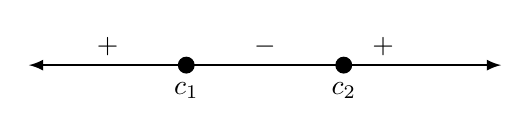
\begin{tikzpicture}[>=latex]
  \draw [thick, <->] (-2,0) -- (4,0);
  \draw [fill] (0.0,0) circle [radius =.1];
  \draw [fill] (2,0) circle [radius =.1];
  \node at (-1,0) [above] {$+$};
  \node at (1,0) [above] {$-$};
  \node at (2.5,0) [above] {$+$};
  \node at (0,-0.1) [below] {$c_1$};
  \node at (2,-0.1) [below] {$c_2$};
  \end{tikzpicture}
\end{center}
\captionsetup{type=figure}%
			\caption{Sign diagram for $\fp$ in Example \ref{ex_sketch1}.}\label{fig:sketchline1fp}
\end{minipage}

From the sign diagram, we see that $f$ is increasing on $(-\infty,c_1)\cup (c_2,\infty)$ (where $fp(x)>0$, and $f$ is decreasing on $(c_1,c_2)$ (where $fp(x)<0$).

Since $fp$ changes from positive to negative at $c_1$, we know that $(c_1,f(c_1))$ is a local maximum, and since $fp$ changes from negative to positive at $c_2$, we know that $(c_2,f(c_2))$ is a local minimum.

\item		Find the possible points of inflection of $f$. We compute $\fpp(x) = 18x-20$. We have 
\[
\fpp(x) = 0 \Rightarrow x= 10/9 \approx 1.111.
\]
\item		Construct a sign diagram for $\fpp$.
We have only one zero for $\fpp$, and we easily see that $\fpp(x)>0$ for $x>10/9$, and $\fpp(x)<0$ for $x<10/9$. The sign diagram for $\fpp$ is given below, with the critical points also indicated for reference:

\noindent\begin{minipage}{\textwidth}
\begin{center}
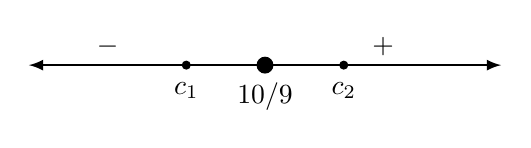
\begin{tikzpicture}[>=latex]
  \draw [thick, <->] (-2,0) -- (4,0);
  \draw [fill] (0.0,0) circle [radius =.05];
  \draw [fill] (2,0) circle [radius =.05];
  \draw [fill] (1,0) circle [radius =.1];
  \node at (-1,0) [above] {$-$};
  \node at (2.5,0) [above] {$+$};
  \node at (0,-0.1) [below] {$c_1$};
  \node at (2,-0.1) [below] {$c_2$};
  \node at (1,-0.1) [below] {$10/9$};
  \end{tikzpicture}
\end{center}
\captionsetup{type=figure}%
			\caption{Sign diagram for $\fpp$ in Example \ref{ex_sketch1}.}\label{fig:sketchline1fpp}
\end{minipage}


\item		We plot the appropriate points on axes as shown in Figure \ref{fig:sketch1}(a) and connect the points with straight lines. In Figure \ref{fig:sketch1}(b) we adjust these lines to demonstrate the proper concavity. Our curve crosses the $y$ axis at $y=5$ and crosses the $x$ axis near $x=-0.424$. In Figure \ref{fig:sketch1}(c) we show a graph of $f$ drawn with a computer program, verifying the accuracy of our sketch.
\end{enumerate}

\mtable{.6}{Sketching $f$ in Example \ref{ex_sketch1}.}{fig:sketch1}
%\mfigure{.8}{Beginning to sketch $f$ in Example \ref{ex_sketch1}.}{fig:sketch1a}{figures/figsketch1a}
%\mfigure{.57}{Adding concavity to the  sketch $f$ in Example \ref{ex_sketch1}.}{fig:sketch1b}{figures/figsketch1b}
%\mfigure{.34}{A computer generated graph of $f$ in Example \ref{ex_sketch1}.}{fig:sketch1}{figures/figsketch1}
}
\vskip-\baselineskip}\\

\example{ex_sketch2}{Curve sketching}{
Sketch $\ds f(x) = \frac{x^2-x-2}{x^2-x-6}$.}
{We again follow the steps outlined in Key Idea \ref{idea:sketch}.

\begin{enumerate}
		\item	In determining the domain, we assume it is all real numbers and look for restrictions. We find that at $x=-2$ and $x=3$, $f(x)$ is not defined. So the domain of $f$ is $D = \{\text{real numbers } x\ | \ x\neq -2,3\}$.
		\item The numerator of $f$ factors as $(x-2)(x+1)$, so $f(x)=0$ for $x=-1$ and $x=2$; these are the $x$-intercepts of $f$. The $y$-intercept is given by $f(0) = 1/3$.
		
Our function has two zeros and two points at which it is undefined. Note that $f(x)$ changes sign at each of these points, so we need to indicate each of them in our sign diagram. We use hollow dots to indicate the points at which $f$ is undefined, giving us the following sign diagram:

\noindent\begin{minipage}{\textwidth}
\begin{center}
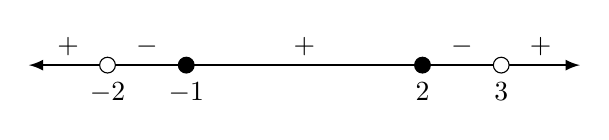
\begin{tikzpicture}[>=latex]
  \draw [thick, <->] (-3,0) -- (4,0);
  \draw [fill=white] (-2.0,0) circle [radius =.1];
  \draw [fill] (-1,0) circle [radius =.1];
  \draw [fill] (2,0) circle [radius =.1];
  \draw [fill=white] (3,0) circle [radius =.1];
  \node at (-2.5,0) [above] {$+$};
  \node at (-1.5,0) [above] {$-$};
  \node at (0.5, 0) [above] {$+$};
  \node at (2.5, 0) [above] {$-$};
  \node at (3.5, 0) [above] {$+$};
  \node at (-2,-0.1) [below] {$-2$};
  \node at (-1,-0.1) [below] {$-1$};
  \node at (2,-0.1) [below] {$2$};
  \node at (3,-0.1) [below] {$3$};
  \end{tikzpicture}
\end{center}
\captionsetup{type=figure}%
			\caption{Sign diagram for $f$ in Example \ref{ex_sketch2}.}\label{fig:sketchline2f}
\end{minipage}		

		\item We see from the sign diagram for $f$ in Figure \ref{fig:sketchline2f} that $f$ has vertical asymptotes at $x=-2$ and $x=3$; moreover, we can deduce the following asymptotic behaviour: at $x=-2$
\[
\lim_{x\to -2^-}f(x) = +\infty \quad \text{ and } \quad \lim_{x\to -2^+}f(x) = -\infty,
\]
and at $x=3$
\[
\lim_{x\to 3^-}f(x) = -\infty \quad \text{ and } \quad 
\lim_{x\to 3^+}f(x) = +\infty.
\]

		\item		There is a horizontal asymptote of $y=1$, as $\ds \lim_{x\to -\infty}f(x) = 1$ and $\ds\lim_{x\to\infty}f(x) =1$.

		\item		To find the critical values of $f$, we first find $\fp(x)$. Using the Quotient Rule, we find 
\[
\fp(x) = \frac{-8x+4}{(x^2+x-6)^2} = \frac{-8x+4}{(x-3)^2(x+2)^2}.
\]
		
		$\fp(x) = 0$ when $x = 1/2$, and $\fp$ is undefined when $x=-2,3$. Since \fp\ is undefined only when $f$ is, these are not critical values. The only critical value is $x=1/2$. The sign diagram for $\fp$ is given as follows:
		
\noindent\begin{minipage}{\textwidth}
\begin{center}
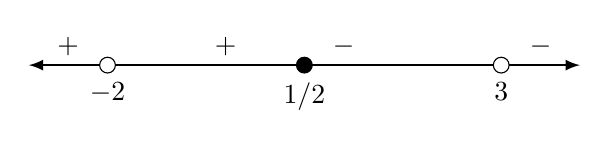
\begin{tikzpicture}[>=latex]
  \draw [thick, <->] (-3,0) -- (4,0);
  \draw [fill=white] (-2.0,0) circle [radius =.1];
  \draw [fill] (0.5,0) circle [radius =.1];
  \draw [fill=white] (3,0) circle [radius =.1];
  \node at (-2.5,0) [above] {$+$};
  \node at (-0.5,0) [above] {$+$};
  \node at (1, 0) [above] {$-$};
  \node at (3.5, 0) [above] {$-$};
  \node at (-2,-0.1) [below] {$-2$};
  \node at (0.5,-0.1) [below] {$1/2$};
  \node at (3,-0.1) [below] {$3$};
  \end{tikzpicture}
\end{center}
\captionsetup{type=figure}%
			\caption{Sign diagram for $\fp$ in Example \ref{ex_sketch2}.}\label{fig:sketchline2fp}
\end{minipage}		
	
	From the sign diagram for $\fp$, we see that $\fp(x)$ changes from positive to negative at $x=1/2$, so we have a local maximum at $(1/2,f(1/2))$. We also see that $f$ is increasing on $(-\infty,-2)\cup(-2,1/2)$ and decreasing on $(1/2,3)\cup (3,\infty)$.
		
		\item		To find the possible points of inflection, we find $\fpp(x)$, again employing the Quotient Rule: 
\[
\fpp(x) = \frac{24x^2-24x+56}{(x-3)^3(x+2)^3}.
\]
		
		\item We find that $\fpp(x)$ is never 0 (setting the numerator equal to 0 and solving for $x$, we find the only roots to this quadratic are imaginary) and \fpp\ is undefined when $x=-2,3$. Thus concavity will possibly only change at $x=-2$ and $x=3$. The sign diagram is given by:

\noindent\begin{minipage}{\textwidth}
\begin{center}
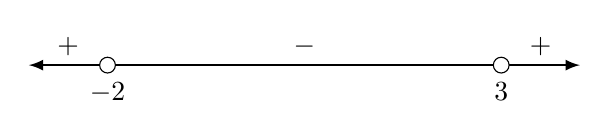
\begin{tikzpicture}[>=latex]
  \draw [thick, <->] (-3,0) -- (4,0);
  \draw [fill=white] (-2.0,0) circle [radius =.1];
  \draw [fill=white] (3,0) circle [radius =.1];
  \node at (-2.5,0) [above] {$+$};
  \node at (0.5, 0) [above] {$-$};
  \node at (3.5, 0) [above] {$+$};
  \node at (-2,-0.1) [below] {$-2$};
  \node at (3,-0.1) [below] {$3$};
  \end{tikzpicture}
\end{center}
\captionsetup{type=figure}%
			\caption{Sign diagram for $\fpp$ in Example \ref{ex_sketch2}.}\label{fig:sketchline2fpp}
\end{minipage}
		
From the sign diagram we see that the graph of $f$ is concave up on $(-\infty,-2)\cup (3,\infty)$ and concave down on $(-2,3)$		
		
	
		\item		In Figure \ref{fig:sketch2}(a), we plot the points from the number line on a set of axes and connect the points with straight lines to get a general idea of what the function looks like (these lines effectively only convey increasing/decreasing information). In Figure \ref{fig:sketch2}(b), we adjust the graph with the appropriate concavity. We also show $f$ crossing the $x$ axis at $x=-1$ and $x=2$.
\end{enumerate}
Figure \ref{fig:sketch2}(c) shows a computer generated graph of $f$, which verifies the accuracy of our sketch.

\enlargethispage{2\baselineskip}

\mtable{.4}{Sketching $f$ in Example \ref{ex_sketch2}.}{fig:sketch2}{%
\begin{tabular}{c}
\myincludegraphics{figures/figsketch2a}\\[10pt]
(a)\\[10pt]
\myincludegraphics{figures/figsketch2b}\\[10pt]
(b)\\[10pt]
\myincludegraphics{figures/figsketch2}\\[10pt]
(c)
\end{tabular}
%\mfigure{.8}{Beginning to sketch $f$ in Example \ref{ex_sketch2}.}{fig:sketch2a}{figures/figsketch2a}
%\mfigure{.57}{Adding concavity to the  sketch $f$ in Example \ref{ex_sketch2}.}{fig:sketch2b}{figures/figsketch2b}
%\mfigure{.34}{A computer generated graph of $f$ in Example \ref{ex_sketch2}.}{fig:sketch2}{figures/figsketch2}
}% ends if/then/else
\vskip-\baselineskip}\pagebreak

\example{ex_sketch3}{Curve sketching}{
Sketch $\ds f(x) = \frac{5(x-2)(x+1)}{x^2+2x+4}.$}
{We again follow Key Idea \ref{idea:sketch}.
	\begin{enumerate}
	\item		We assume that the domain of $f$ is all real numbers and consider restrictions. The only restrictions come when the denominator is 0, but this never occurs. Therefore the domain of $f$ is all real numbers, $\mathbb{R}$.
\item The $x$-intercepts of $f$ are $(-1,0)$, and $(2,0)$, and the $y$-intercept is $(0,-5/2)$. The sign diagram of $f$ is given below:

\noindent\begin{minipage}{\textwidth}
\begin{center}
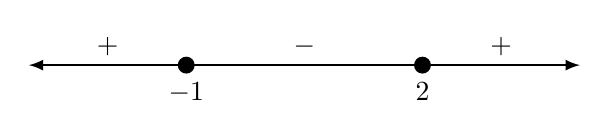
\begin{tikzpicture}[>=latex]
  \draw [thick, <->] (-3,0) -- (4,0);
  \draw [fill] (-1,0) circle [radius =.1];
  \draw [fill] (2,0) circle [radius =.1];
  \node at (-2,0) [above] {$+$};
  \node at (0.5, 0) [above] {$-$};
  \node at (3, 0) [above] {$+$};
  \node at (-1,-0.1) [below] {$-1$};
  \node at (2,-0.1) [below] {$2$};
  \end{tikzpicture}
\end{center}
\captionsetup{type=figure}%
			\caption{Sign diagram for $f$ in Example \ref{ex_sketch3}.}\label{fig:sketchline3f}
\end{minipage}	

    \item Since the domain of $f$ is $\mathbb{R}$, there are no vertical asymptotes.
    
    \item		We have a horizontal asymptote of $y=5$, as $\ds \lim_{x\to-\infty}f(x) = \lim_{x\to\infty}f(x) = 5$.
    
	\item		We find the critical values of $f$ by setting $\fp(x)=0$ and solving for $x$. We find 
\[
\fp(x) = \frac{15x(x+4)}{(x^2+2x+4)^2} \quad \Rightarrow \quad \fp(x) = 0 \text{ when } \ x=-4,0.
\]

	\item The sign diagram for $\fp$ is given by:
	
\noindent\begin{minipage}{\textwidth}
\begin{center}
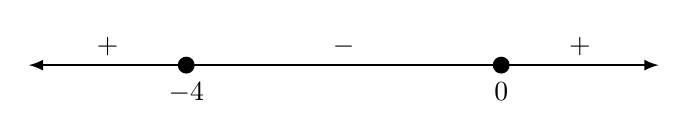
\begin{tikzpicture}[>=latex]
  \draw [thick, <->] (-6,0) -- (2,0);
  \draw [fill] (-4,0) circle [radius =.1];
  \draw [fill] (0,0) circle [radius =.1];
  \node at (-5,0) [above] {$+$};
  \node at (-2, 0) [above] {$-$};
  \node at (1, 0) [above] {$+$};
  \node at (-4,-0.1) [below] {$-4$};
  \node at (0,-0.1) [below] {$0$};
  \end{tikzpicture}
\end{center}
\captionsetup{type=figure}%
			\caption{Sign diagram for $\fp$ in Example \ref{ex_sketch3}.}\label{fig:sketchline3fp}
\end{minipage}	

From the sign diagram, we see that $\fp(x)$ changes from positive to negative at $x=-4$, so $(-4,f(-4))$ is a relative maximum, and $\fp(x)$ changes from negative to positive at $x=0$, so $(0,f(0))$ is a relative minimum. We also see that $f$ is increasing on $(-\infty,-4)\cup (0,\infty)$, and decreasing on $(-4,0)$.
	
	\item		We find the possible points of inflection by solving $\fpp(x) = 0$ for $x$. We find
\[
\fpp(x) = -\frac{30x^3+180x^2-240}{(x^2+2x+4)^3} .
\]
 The cubic in the numerator does not factor very ``nicely.'' We instead approximate the roots (with the help of a computer) at $c_1= -5.759$, $c_2=-1.305$ and $c_3=1.064$. The sign diagram for $\fpp$ is given by:
 
\noindent\begin{minipage}{\textwidth}
\begin{center}
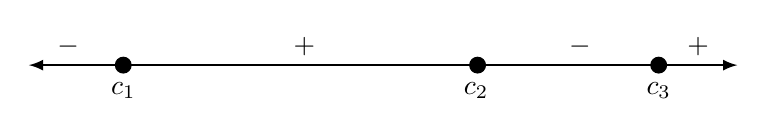
\begin{tikzpicture}[>=latex]
  \draw [thick, <->] (-7,0) -- (2,0);
  \draw [fill] (-5.8,0) circle [radius =.1];
  \draw [fill] (-1.3,0) circle [radius =.1];
  \draw [fill] (1,0) circle [radius =.1];
  \node at (-6.5,0) [above] {$-$};
  \node at (-3.5, 0) [above] {$+$};
  \node at (0, 0) [above] {$-$};
  \node at (1.5, 0) [above] {$+$};
  \node at (-5.8,-0.1) [below] {$c_1$};
  \node at (-1.32,-0.1) [below] {$c_2$};
  \node at (1,-0.1) [below] {$c_3$};
  \end{tikzpicture}
\end{center}
\captionsetup{type=figure}%
			\caption{Sign diagram for $\fpp$ in Example \ref{ex_sketch3}.}\label{fig:sketchline3fpp}
\end{minipage}	

\enlargethispage{\baselineskip}
	
	\item		In Figure \ref{fig:sketch3}(a) we plot the significant points from the number line as well as the two roots of $f$, $x=-1$ and $x=2$, and connect the points with straight lines to get a general impression about the graph. In Figure \ref{fig:sketch3}(b), we add concavity. Figure \ref{fig:sketch3}(c) shows a computer generated graph of $f$, affirming our results.		
	\end{enumerate}
	
\mtable{.5}{Sketching $f$ in Example \ref{ex_sketch3}.}{fig:sketch3}{%
\begin{tabular}{c}
\myincludegraphics{figures/figsketch3a}\\[10pt]
(a)\\[10pt]
\myincludegraphics{figures/figsketch3b}\\[10pt]
(b)\\[10pt]
\myincludegraphics{figures/figsketch3}\\[10pt]
(c)
\end{tabular}
%\mfigure{.8}{Beginning to sketch $f$ in Example \ref{ex_sketch3}.}{fig:sketch3a}{figures/figsketch3a}
%\mfigure{.57}{Adding concavity to the  sketch $f$ in Example \ref{ex_sketch3}.}{fig:sketch3b}{figures/figsketch3b}
%\mfigure{.34}{A computer generated graph of $f$ in Example \ref{ex_sketch3}.}{fig:sketch3}{figures/figsketch3}
}% ends if/then/else
\vskip-\baselineskip}\pagebreak

In each of our examples, we found a few, significant points on the graph of $f$ that corresponded to changes in increasing/decreasing or concavity. We connected these points with straight lines, then adjusted for concavity, and finished by showing a very accurate, computer generated graph. 

Why are computer graphics so good? It is not because computers are ``smart\-er'' than we are. Rather, it is largely because computers are much faster at computing than we are. In general, computers graph functions much like most students do when first learning to draw graphs: they plot equally spaced points, then connect the dots using lines. By using lots of points, the connecting lines are short and the graph looks smooth. 

This does a fine job of graphing in most cases (in fact, this is the method used for many graphs in this text). However, in regions where the graph is very ``curvy,'' this can generate noticeable sharp edges on the graph unless a large number of points are used. High quality computer algebra systems, such as \textit{Mathematica}, use special algorithms to plot lots of points only where the graph is ``curvy.''

In Figure \ref{fig:mathematica_sinx}, a graph of $y=\sin x$ is given, generated by \textit{Mathematica}. The small points represent each of the places \textit{Mathematica} sampled the function. Notice how at the ``bends'' of $\sin x$, lots of points are used; where $\sin x$ is relatively straight, fewer points are used. (Many points are also used at the endpoints to ensure the ``end behaviour'' is accurate.) 

\vskip\baselineskip
\noindent%
\begin{minipage}{\textwidth}\centering
\includegraphics{figures/figmathematica_sinx}
\captionsetup{type=figure}%
			\caption{A graph of $y=\sin x$ generated by \textit{Mathematica}.}\label{fig:mathematica_sinx}
\end{minipage}
\vskip\baselineskip

How does \textit{Mathematica} know where the graph is ``curvy''? Calculus. When we study \textit{curvature} in a later chapter, we will see how the first and second derivatives of a function work together to provide a measurement of ``curviness.'' \textit{Mathematica} employs algorithms to determine regions of ``high curvature'' and plots extra points there.

Again, the goal of this section is not ``How to graph a function when there is no computer to help.'' Rather, the goal is ``Understand that the shape of the graph of a function is largely determined by understanding the behaviour of the function at a few key places.'' In Example \ref{ex_sketch3}, we were able to accurately sketch a complicated graph using only 5 points and knowledge of asymptotes!

There are many applications of our understanding of derivatives beyond curve sketching. The next chapter explores some of these applications, demonstrating just a few kinds of problems that can be solved with a basic knowledge of differentiation. 

\printexercises{exercises/03_05_exercises}

%%\addtocounter{chapter}{3}
%
%\clearpage{\pagestyle{empty}\cleardoublepage}
%\chapter{Applications of the Derivative}\label{chapter:deriv_apps}
%\thispagestyle{empty}
%
%\input{text/04_NewtonsMethod}
%\input{text/04_Related_Rates}
%\input{text/04_Optimization}
%\input{text/04_Differentials}


%\addtocounter{chapter}{5}

%\clearpage{\pagestyle{empty}\cleardoublepage}

%\setcounterref{definitioncounter}{lastdefcount1}
%\addtocounter{definitioncounter}{-1}
%\setcounterref{theoremcounter}{lastthmcount1}
%\addtocounter{theoremcounter}{-1}
%\setcounterref{keyideacounter}{lastideacount1}
%\addtocounter{keyideacounter}{-1}
%\setcounterref{examplecounter}{lastexamplecount1}
%\addtocounter{examplecounter}{-1}
%\setcounter{page}{189}
%\thispagestyle{empty}

%\chapter{Integration}\label{chapter:integration}
%\addtocontents{toc}{\protect\enlargethispage{2\baselineskip}}
%\thispagestyle{empty}
%\setcounterpageref{page}{lastdefcount1}
%\addtocounter{page}{4}
%\input{text/05_Antiderivatives}
%\addtocontents{toc}{\protect\thispagestyle{empty}}
%\input{text/05_Definite_Integral}
%\input{text/05_Riemann_Sums}
%\input{text/05_FTC}
%\input{text/05_Numerical_Integration}


%%\addtocounter{chapter}{5}

%\clearpage{\pagestyle{empty}\cleardoublepage}
%\chapter{Techniques of Antidifferentiation}\label{chapter:anti_tech}
%\thispagestyle{empty}

%\input{text/06_Substitution}
%\input{text/06_Int_By_Parts}
%\input{text/06_Trigonometric_Integrals}
%\section{Trigonometric Substitution}\label{sec:trig_sub}

In Section \ref{I-sec:def_int} we defined the definite integral as the ``signed area under the curve.'' In that section we had not yet learned the Fundamental Theorem of Calculus, so we only evaluated special definite integrals which described nice, geometric shapes. For instance, we were able to evaluate
\begin{equation}
\int_{-3}^3\sqrt{9-x^2}\ dx = \frac{9\pi}{2}\label{eq:trigsub1}
\end{equation}
 as we recognized that $f(x) = \sqrt{9-x^2}$ described the upper half of a circle with radius 3. 

We have since learned a number of integration techniques, including Substitution and Integration by Parts, yet we are still unable to evaluate the above integral without resorting to a geometric interpretation. This section introduces Trigonometric Substitution, a method of integration that fills this gap in our integration skill. This technique works on the same principle as Substitution as found in Section \ref{sec:substitution}, though it can feel ``backward.'' In Section \ref{sec:substitution}, we set $u=f(x)$, for some function $f$, and replaced $f(x)$ with $u$. In this section, we will set $x=f(\theta)$, where $f$ is a trigonometric function, then replace $x$ with $f(\theta)$. 

We start by demonstrating this method in evaluating the integral in Equation \eqref{eq:trigsub1}. After the example, we will generalize the method and give more examples.\\
\enlargethispage{3\baselineskip}

\example{ex_trigsub1}{Using Trigonometric Substitution}{
Evaluate $\ds \int_{-3}^3\sqrt{9-x^2}\ dx$.}
{We begin by noting that $9\sin^2\theta + 9\cos^2\theta = 9$, and hence $9\cos^2\theta = 9-9\sin^2\theta$. If we let $x=3\sin\theta$, then $9-x^2 = 9-9\sin^2\theta = 9\cos^2\theta$. 

Setting $x=3\sin \theta$ gives  $dx = 3\cos\theta\ d\theta$. We are almost ready to substitute. We also wish to change our bounds of integration. The bound $x=-3$ corresponds to $\theta = -\pi/2$ (for when $\theta = -\pi/2$, $x=3\sin \theta = -3$). Likewise, the bound of $x=3$ is replaced by the bound $\theta = \pi/2$. Thus
\begin{align*}
\int_{-3}^3\sqrt{9-x^2}\ dx &= \int_{-\pi/2}^{\pi/2} \sqrt{9-9\sin^2\theta} (3\cos\theta)\ d\theta \\
		&= \int_{-\pi/2}^{\pi/2} 3\sqrt{9\cos^2\theta} \cos\theta\ d\theta \\
		&=\int_{-\pi/2}^{\pi/2} 3|3\cos \theta| \cos\theta\ d\theta.
		\intertext{On $[-\pi/2,\pi/2]$, $\cos \theta$ is always positive, so we can drop the absolute value bars, then employ a power--reducing formula:}
\end{align*}
\begin{align*}
			&= \int_{-\pi/2}^{\pi/2} 9\cos^2 \theta\ d\theta\\
			&= \int_{-\pi/2}^{\pi/2} \frac{9}{2}\big(1+\cos(2\theta)\big)\ d\theta\\
			& = \frac92 \big(\theta +\frac12\sin(2\theta)\big)\Bigg|_{-\pi/2}^{\pi/2}= \frac92\pi.
\end{align*}
This matches our answer from before.
}\\

We now describe in detail Trigonometric Substitution. This method excels when dealing with integrands that contain $\sqrt{a^2-x^2}$, $\sqrt{x^2-a^2}$ and $\sqrt{x^2+a^2}$. The following Key Idea outlines the procedure for each case, followed by more examples. Each right triangle acts as a reference to help us understand the relationships between $x$ and $\theta$.
\enlargethispage{2\baselineskip}

\setboxwidth{100pt}
\hskip-100pt%
\noindent\begin{minipage}{\linewidth+100pt}
\keyidea{idea:trigsub}{Trigonometric Substitution}
{For the three cases below, we assume that $a>0$.
\begin{enumerate}
	\item[(a)] \noindent%
		\begin{minipage}[t]{.6\linewidth}%
		For integrands containing $\sqrt{a^2-x^2}$:\index{integration!trig. subst.}\\[5pt]
		Let $x=a\sin\theta$, \qquad $dx = a\cos\theta\ d\theta$\\[5pt]	
	Thus $\theta = \sin^{-1}(x/a)$, for $-\pi/2\leq \theta\leq \pi/2$. \\[5pt]	
	On this interval, $\cos\theta\geq 0$, so\\[5pt]	
	$\sqrt{a^2-x^2} = a\cos\theta$
		\end{minipage}\qquad
	\begin{minipage}[t]{.4\linewidth}\vskip 0pt
		\includegraphics{figures/figtrigsub_intro1}
		\end{minipage}
		
	\item[(b)] \noindent
	\begin{minipage}[t]{.6\linewidth}
		For integrands containing $\sqrt{x^2+a^2}$:\\[5pt]
		Let $x=a\tan\theta$, \qquad $dx = a\sec^2\theta\ d\theta$\\[5pt]	
	Thus $\theta = \tan^{-1}(x/a)$, for $-\pi/2 < \theta < \pi/2$. \\[5pt]	
	On this interval, $\sec\theta> 0$, so\\[5pt]	
	$\sqrt{x^2+a^2} = a\sec\theta$
		\end{minipage}\qquad
	\begin{minipage}[t]{.4\linewidth}\vskip 0pt
		\includegraphics{figures/figtrigsub_intro3}
		\end{minipage}
		
	\item[(c)] \noindent
	\begin{minipage}[t]{.6\linewidth}
		For integrands containing $\sqrt{x^2-a^2}$:\\[5pt]
		Let $x=a\sec\theta$, \qquad $dx = a\sec\theta\tan\theta\ d\theta$\\[5pt]	
	Thus $\theta = \sec^{-1}(x/a)$. Note that $\sqrt{x^2-a^2}$ is defined for $x\geq a$ or $x\leq -a$.\\
	 If $x\geq a$, then $x/a\geq 1$ and $0\leq\theta<\pi/2$; if $x<-a$, then $x/a \leq -1$ and $\pi\leq\theta< \frac{3\pi}{2}$.\\[5pt]	
	On these intervals, $\tan\theta\geq 0$, so\\[5pt]	
	$\sqrt{x^2-a^2} = a\tan\theta$
		\end{minipage}\qquad
	\begin{minipage}[t]{.4\linewidth}\vskip 0pt
		\includegraphics{figures/figtrigsub_intro2}
		\end{minipage}	
\end{enumerate}
}
\end{minipage}
\restoreboxwidth
\vskip \baselineskip

\example{ex_trigsub3}{Using Trigonometric Substitution}{
Evaluate $\ds \int \frac{1}{\sqrt{5+x^2}}\ dx.$}
{Using Key Idea \ref{idea:trigsub}(b), we recognize $a=\sqrt{5}$ and  set $x= \sqrt{5}\tan \theta$. This makes $dx = \sqrt{5}\sec^2\theta\ d\theta$. We will use the fact that $\sqrt{5+x^2} = \sqrt{5+5\tan^2\theta} = \sqrt{5\sec^2\theta} = \sqrt{5}\sec\theta.$ Substituting, we have:
\begin{align*}
\int \frac{1}{\sqrt{5+x^2}}\ dx &= \int \frac{1}{\sqrt{5+5\tan^2\theta}}\sqrt{5}\sec^2\theta\ d\theta \\
			&= \int \frac{\sqrt{5}\sec^2\theta}{\sqrt{5}\sec\theta} \ d\theta\\
			&= \int \sec\theta\ d\theta\\
			&= \ln\big|\sec\theta+\tan\theta\big|+C.
\end{align*}
While the integration steps are over, we are not yet done. The original problem was stated in terms of $x$, whereas our answer is given in terms of $\theta$. We must convert back to $x$.

The reference triangle given in Key Idea \ref{idea:trigsub}(b) helps. With $x=\sqrt{5}\tan\theta$, we have 
\[
\tan \theta = \frac x{\sqrt{5}}\quad \text{and}\quad \sec\theta = \frac{\sqrt{x^2+5}}{\sqrt{5}}.
\]
This gives
\begin{align*}
\int \frac{1}{\sqrt{5+x^2}}\ dx &= \ln\big|\sec\theta+\tan\theta\big|+C \\
     &= \ln\left|\frac{\sqrt{x^2+5}}{\sqrt{5}}+ \frac x{\sqrt{5}}\right|+C.
\end{align*}
We can leave this answer as is, or we can use a logarithmic identity to simplify it. Note:
\begin{align*}
\ln\left|\frac{\sqrt{x^2+5}}{\sqrt{5}}+ \frac x{\sqrt{5}}\right|+C &= \ln\left|\frac{1}{\sqrt{5}}\big(\sqrt{x^2+5}+ x\big)\right|+C \\
   &= \ln\left|\frac{1}{\sqrt{5}}\right| + \ln\big|\sqrt{x^2+5}+ x\big|+C\\
	&=	\ln\big|\sqrt{x^2+5}+ x\big|+C,
\end{align*}
where the $\ln\big(1/\sqrt{5}\big)$ term is absorbed into the constant $C$. (In Section \ref{sec:hyperbolic} we will learn another way of approaching this problem.)
}\\

\example{ex_trigsub2}{Using Trigonometric Substitution}{
Evaluate $\ds \int \sqrt{4x^2-1}\ dx$.}
{We start by rewriting the integrand so that it looks like $\sqrt{x^2-a^2}$ for some value of $a$:
\begin{align*}
\sqrt{4x^2-1} &= \sqrt{4\left(x^2-\frac14\right)}\\
		&= 2\sqrt{x^2-\left(\frac12\right)^2}.
\end{align*}
So we have $a=1/2$, and following Key Idea \ref{idea:trigsub}(c), we set $x= \frac12\sec\theta$, and hence $dx = \frac12\sec\theta\tan\theta\ d\theta$. %The Key Idea also shows that $\sqrt{x^2-1/2^2} = \frac12\tan\theta$. 
We now rewrite the integral with these substitutions:
\begin{align*}
\int \sqrt{4x^2-1}\ dx &= \int 2\sqrt{x^2-\left(\frac12\right)^2}\ dx\\
			&= \int 2\sqrt{\frac14\sec^2\theta - \frac14}\left(\frac12\sec\theta\tan\theta\right)\ d\theta\\
			&=\int \sqrt{\frac14(\sec^2\theta-1)}\Big(\sec\theta\tan\theta\Big)\ d\theta\\
			&=\int\sqrt{\frac14\tan^2\theta}\Big(\sec\theta\tan\theta\Big)\ d\theta\\
			&=\int \frac12\tan^2\theta\sec\theta\ d\theta\\
			&=\frac12\int \Big(\sec^2\theta-1\Big)\sec\theta\ d\theta\\
			&=\frac12\int \big(\sec^3\theta - \sec\theta\big)\ d\theta.
\end{align*}
We integrated $\sec^3\theta$ in Example \ref{ex_trigint6}, finding its antiderivatives to be
\[
\int \sec^3\theta\ d\theta = \frac12\Big(\sec \theta\tan \theta + \ln|\sec \theta+\tan \theta|\Big)+C.
\]
\enlargethispage{2\baselineskip}
Thus
\begin{align*}
\int \sqrt{4x^2-1}\ dx &=\frac12\int \big(\sec^3\theta - \sec\theta\big)\ d\theta\\
			&= \frac12\left(\frac12\Big(\sec \theta\tan \theta + \ln|\sec \theta+\tan \theta|\Big) -\ln|\sec \theta + \tan\theta|\right) + C\\
			%\end{align*}
			%\begin{align*}
			&= \frac14\left(\sec\theta\tan\theta -\ln|\sec\theta+\tan\theta|\right)+C.
\end{align*}
We are not yet done. Our original integral is given in terms of $x$, whereas our final answer, as given, is in terms of $\theta$. We need to rewrite our answer in terms of $x$. With $a=1/2$, and $x=\frac12\sec\theta$, the reference triangle in Key Idea \ref{idea:trigsub}(c) shows that 
\[
\tan \theta = \sqrt{x^2-1/4}\Big/(1/2) = 2\sqrt{x^2-1/4}\quad \text{and}\quad \sec\theta = 2x.
\]
Thus\small 
\begin{align*}
\frac14\Big(\sec\theta\tan\theta -\ln\big|\sec\theta+\tan\theta\big|\Big)+C &=
				\frac14\Big(2x\cdot 2\sqrt{x^2-1/4} - \ln\big|2x + 2\sqrt{x^2-1/4}\big|\Big)+C\\
				&= \frac14\Big(4x\sqrt{x^2-1/4} - \ln\big|2x + 2\sqrt{x^2-1/4}\big|\Big)+C.
\end{align*}
\normalsize 
The final answer is given in the last line above, repeated here:
\[
\int \sqrt{4x^2-1}\ dx = \frac14\Big(4x\sqrt{x^2-1/4} - \ln\big|2x + 2\sqrt{x^2-1/4}\big|\Big)+C.
\]
}\\

\example{ex_trigsub4}{Using Trigonometric Substitution}{
Evaluate $\ds \int \frac{\sqrt{4-x^2}}{x^2}\ dx$.}
{We use Key Idea \ref{idea:trigsub}(a) with $a=2$, $x=2\sin \theta$, $dx = 2\cos \theta$ and hence $\sqrt{4-x^2} = 2\cos\theta$. This gives
\begin{align*}
\int \frac{\sqrt{4-x^2}}{x^2}\ dx &= \int \frac{2\cos\theta}{4\sin^2\theta}(2\cos\theta)\ d\theta\\
		&= \int \cot^2\theta\ d\theta\\
		&=	\int (\csc^2\theta -1)\ d\theta\\
		&= -\cot\theta -\theta + C.
\end{align*}
We need to rewrite our answer in terms of $x$. Using the reference triangle found in Key Idea \ref{idea:trigsub}(a), we have $\cot\theta = \sqrt{4-x^2}/x$ and $\theta = \sin^{-1}(x/2)$. Thus
\[
\int \frac{\sqrt{4-x^2}}{x^2}\ dx = -\frac{\sqrt{4-x^2}}x-\sin^{-1}\left(\frac x2\right) + C.
\]
}\\

Trigonometric Substitution can be applied in many situations, even those not of the form $\sqrt{a^2-x^2}$, $\sqrt{x^2-a^2}$ or $\sqrt{x^2+a^2}$. In the following example, we apply it to an integral we already know how to handle.\\

\example{ex_trigsub5}{Using Trigonometric Substitution}{
Evaluate $\ds \int\frac1{x^2+1}\ dx$.}
{We know the answer already as $\tan^{-1}x+C$. We apply Trigonometric Substitution here to show that we get the same answer without inherently relying on knowledge of the derivative of the arctangent function.

Using Key Idea \ref{idea:trigsub}(b), let $x=\tan\theta$, $dx=\sec^2\theta\ d\theta$ and note that $x^2+1 = \tan^2\theta+1 = \sec^2\theta$. Thus
\begin{align*}
\int \frac1{x^2+1}\ dx &= \int \frac{1}{\sec^2\theta}\sec^2\theta\ d\theta \\
			&= \int 1\ d\theta\\
			&= \theta + C.
\end{align*}
Since $x=\tan \theta$, $\theta = \tan^{-1}x$, and we conclude that $\ds \int\frac1{x^2+1}\ dx = \tan^{-1}x+C.$
}\\

The next example is similar to the previous one in that it does not involve a square--root. It shows how several techniques and identities can be combined to obtain a solution.\\

\example{ex_trigsub7}{Using Trigonometric Substitution}{
Evaluate $\ds\int\frac1{(x^2+6x+10)^2}\ dx.$
}
{We start by completing the square, then make the substitution $u=x+3$, followed by the trigonometric substitution of $u=\tan\theta$:
\begin{align}
\int \frac1{(x^2+6x+10)^2}\ dx =\int \frac1{\big((x+3)^2+1\big)^2}\ dx&= \int \frac1{(u^2+1)^2}\ du. \notag
\intertext{Now make the substitution $u=\tan\theta$, $du=\sec^2\theta\ d\theta$:}
   &=	\int \frac1{(\tan^2\theta+1)^2}\sec^2\theta\ d\theta\notag\\
	&= \int\frac 1{(\sec^2\theta)^2}\sec^2\theta\ d\theta\notag\\
	&= \int \cos^2\theta\ d\theta.\notag
	\intertext{Applying a power reducing formula, we have}
	&= \int \left(\frac12 +\frac12\cos(2\theta)\right)\ d\theta \notag\\
	&= \frac12\theta + \frac14\sin(2\theta) + C.\label{eq:extrigsub7}
\end{align}
We need to return to the variable $x$. As $u=\tan\theta$, $\theta = \tan^{-1}u$. Using the identity $\sin(2\theta) = 2\sin\theta\cos\theta$ and using the reference triangle found in Key Idea \ref{idea:trigsub}(b), we have 
\[
\frac14\sin(2\theta) = \frac12\frac u{\sqrt{u^2+1}}\cdot\frac 1{\sqrt{u^2+1}} = \frac12\frac u{u^2+1}.
\]
Finally, we return to $x$ with the substitution $u=x+3$. We start with the expression in Equation \eqref{eq:extrigsub7}:
\begin{align*}
\frac12\theta + \frac14\sin(2\theta) + C &= \frac12\tan^{-1}u + \frac12\frac{u}{u^2+1}+C\\
				&= \frac12\tan^{-1}(x+3) + \frac{x+3}{2(x^2+6x+10)}+C.
\end{align*}
Stating our final result in one line,
\[
\int\frac1{(x^2+6x+10)^2}\ dx=\frac12\tan^{-1}(x+3) + \frac{x+3}{2(x^2+6x+10)}+C.
\]
}\\


Our last example returns us to definite integrals, as seen in our first example. Given a definite integral that can be evaluated using Trigonometric Substitution, we could first evaluate the corresponding indefinite integral (by changing from an integral in terms of $x$ to one in terms of $\theta$, then converting back to $x$) and then evaluate using the original bounds. It is much more straightforward, though, to change the bounds as we substitute.\\

\example{ex_trigsub6}{Definite integration and Trigonometric Substitution}{
Evaluate $\ds\int_0^5\frac{x^2}{\sqrt{x^2+25}}\ dx$.
}
{Using Key Idea \ref{idea:trigsub}(b), we set $x=5\tan\theta$, $dx = 5\sec^2\theta\ d\theta$, and note that $\sqrt{x^2+25} = 5\sec\theta$. As we substitute, we can also change the bounds of integration.

The lower bound of the original integral is $x=0$. As $x=5\tan\theta$, we solve for $\theta$ and find $\theta = \tan^{-1}(x/5)$. Thus the new lower bound is $\theta = \tan^{-1}(0) = 0$. The original upper bound is $x=5$, thus the new upper bound is $\theta = \tan^{-1}(5/5) = \pi/4$. 

Thus we have 
\begin{align*}
\int_0^5\frac{x^2}{\sqrt{x^2+25}}\ dx &= \int_0^{\pi/4} \frac{25\tan^2\theta}{5\sec\theta}5\sec^2\theta\ d\theta\\
		&= 25\int_0^{\pi/4} \tan^2\theta\sec\theta\ d\theta.
\end{align*}
We encountered this indefinite integral in Example \ref{ex_trigsub2} where we found 
\[
\int \tan^2\theta\sec\theta \ d\theta = \frac12\big(\sec\theta\tan\theta-\ln|\sec\theta+\tan\theta|\big).
\]
So
\begin{align*}
25\int_0^{\pi/4} \tan^2\theta\sec\theta\ d\theta &= \frac{25}2\big(\sec\theta\tan\theta-\ln|\sec\theta+\tan\theta|\big)\Bigg|_0^{\pi/4}\\
&= \frac{25}2\big(\sqrt2-\ln(\sqrt2+1)\big)\\
&\approx 6.661.
\end{align*}
\vskip-1.5\baselineskip
}\\

\enlargethispage{3\baselineskip}
The following equalities are very useful when evaluating integrals using Trigonometric Substitution. 

\keyidea{idea:useful_trigsub}{Useful Equalities with Trigonometric Substitution}
{\begin{enumerate}
	\item	$\sin(2\theta) = 2\sin\theta\cos\theta$
	\item	$\cos(2\theta) = \cos^2\theta - \sin^2\theta = 2\cos^2\theta-1 = 1-2\sin^2\theta$
	\item $\ds \int \sec^3\theta\ d\theta = \frac12\Big(\sec \theta\tan \theta + \ln\big|\sec \theta+\tan \theta\big|\Big)+C$
	\item	$\ds \int \cos^2\theta\ d\theta = \int \frac12\big(1+\cos(2\theta)\big)\ d\theta = \frac12\big(\theta+\sin\theta\cos\theta\big)+C.$
\end{enumerate}
}

%\subsection*{Hyperbolic substitution}
%For integrands containing terms of the form $\sqrt{x^2+a^2}$ or $\sqrt{x^2-a^2}$, it is also possible to make use of \sword{hyperbolic substitution} \index{substitution ! hyperbolic}. Recall from Section \ref{sec:hyperbolic} of the Math 1560 textbook that the hyperbolic functions are defined by
%\[
%\cosh(x) = \frac{e^x+e^{-x}}{2} \quad \text{ and } \quad \sinh(x) %= \frac{e^x-e^{-x}}{2},
%\]
%with $\tanh(x) = \dfrac{\sinh(x)}{\cosh(x)}$, and so on. Recall that the hyperbolic functions satisfy the identity
%\[
%\cosh^2(x)-\sinh^2(x)  = 1.
%\]
%If we're given $\sqrt{x^2+a^2}$, we can let $x=a\sinh(t)$, then
%\[
%x^2+a^2 = (a\sinh(t))^2+a^2 = a^2(\sinh^2(t)+1) = a^2\cosh^2(t),
%\]
%and $dx = a\cosh(t)\,dt$. Since $\cosh(t)>0$ for all real numbers $t$, we have $\sqrt{a^2+x^2}=\cosh(t)$.

%If we're given $\sqrt{x^2-a^2}$, we can let $x=a\cosh(t)$; then
%\[
%x^2-a^2 = (a\cosh(t))^2-a^2 = a^2(\cosh^2(t)-1) = a^2\sinh^2(t),
%\]
%and $dx = a\sinh(t)$. (One of the convenient aspects of working with hyperbolic functions is that there are no signs to worry about when taking derivatives.)
%Note that $\cosh(t)>0$ for all $t$, so the substitution $x=a\cosh(t)$ works in the case that $x\geq a>0$. In this case, $\sqrt{x^2-a^2} = a\sinh(t)$. For $x<-a<0$, technically we would need to let $x=-a\cosh(t)$. We illustrate this method with a couple of examples.\\

%\example{ex_hypsub1}{Using hyperbolic substitution}{
%Use hyperbolic substitution to evaluate the integral $\displaystyle \int\frac{3}{\sqrt{x^2+4}}\,dx$.
%}
%{
%Here we encounter the form $\sqrt{x^2+4} = \sqrt{x^2+2^2}$, so we use the substitution $x=2\sinh(t)$, or $t=\sinh^{-1}(x/2)$. This gives us
%\[
%\sqrt{x^2+4} = \sqrt{4\sinh^2(t)+4} = \sqrt{4\cosh^2(t)}=2\cosh(t),
%\]
%and $dx = 4\cosh(t)\,dt$. Substituting these into the integral, we have
%\begin{align*}
%\int\frac{3}{\sqrt{x^2+4}}\,dx &= \int \frac{3(2\cosh(t))}{2\cosh(t)}\,dt\\
%& = \int 3 \,dt = 3t+C\\
%& = 3\sinh^{-1}\left(\frac{x}{2}\right)+C.
%\end{align*}

%Of course, we could also evaluate the integral using the substitution $x=2\tan\theta$. In this case, the hyperbolic substitution turns out to be much simpler. Let's go through the details to confirm this. If $x=2\tan\theta$, then we have $dx = 2\sec^2\theta\,d\theta$, and
%\[
%\sqrt{x^2+4} = \sqrt{4\tan^2\theta+4} = \sqrt{4\sec^2\theta} = 2\sec\theta.
%\]
%In terms of $\theta$, our integral is
%\begin{align*}
%\int\frac{3}{\sqrt{x^2+4}}\,dx & = \int \frac{3(2\sec^2\theta)}{2\sec\theta}\,d\theta\\
% & = \int 3\sec\theta\,d\theta\\
% & = 3\ln\lvert \sec\theta +\tan\theta\rvert+C\\
% & = 3\ln\left( \frac{\sqrt{x^2+4}}{2} + \frac{x}{2}\right) +C.
%\end{align*}
%(Note that since $\sqrt{x^2+4}>x$ for all values of $x$, we can drop the absolute value in the argument of the logarithm.)

%The answer using the hyperbolic substitution certainly looks simpler, and it was easier to obtain, but are the two results equivalent? That is, is it true that
%\[
%\sinh^{-1}\left(\frac{x}{2}\right) = \ln\left(\frac{\sqrt{x^2+4}+x}{2}\right)?
%\]
%To check, let's take the hyperbolic sine of both sides. On the left, this yields $\frac{x}{2}$. On the right, we get
%\begin{align*}
%\sinh\left[\ln\left(\frac{\sqrt{x^2+4}+x}{2}\right)\right] & = \frac{1}{2}\left[e^{\ln\left(\frac{\sqrt{x^2+4}+x}{2}\right)}-e^{\ln\left(\frac{\sqrt{x^2+4}+x}{2}\right)}\right]\\
%& = \frac{1}{2}\left[\frac{\sqrt{x^2+4}+x}{2}-\frac{2}{\sqrt{x^2+4}+x}\right]\\
%& = \frac{1}{2}\left[\frac{(\sqrt{x^2+4}+x)^2-4}{2(\sqrt{x^2+4}+x)}\right]\\
%& = \frac{1}{4}\left[\frac{(x^2+4)+2x\sqrt{x^2+4}+x^2-4}{\sqrt{x^2+4}+x}\right]\\
%& = \frac{1}{4}\left[\frac{2x(\sqrt{x^2+4}+x)}{\sqrt{x^2+4}+x}\right]\\
%& = \frac{x}{2},
%\end{align*}
%so the results agree!
%}\\

%\example{ex_hypsub2}{Using hyperbolic substitution}{
%Evaluate the integral $\displaystyle \int\frac{x^2}{\sqrt{x^2-16}}\,dx$ using a hyperbolic substitution.
%}
%{Once again, we \textit{could} use the substitution $x=4\sec\theta$, but doing so leads us to a $\sec^3\theta$ integral, and those are never fun. (Feel free to try it this way) Instead, we decide to read (and follow) the instructions, and use a hyperbolic substitution.

%The form $\sqrt{x^2-16}$ tells us that we should try the substitution $x=4\cosh(t)$.  This gives us $dx = 4\sinh(t)$, and
% \[
% \sqrt{x^2-16} = \sqrt{16(\cosh^2(t)-1)} = \sqrt{16\sinh^2(t)} = 4\sinh(t).
% \]
% Thus,
% \[
% \int \frac{x^2}{\sqrt{x^2-16}}\,dx = \int \frac{16\cosh^2(t)}{4\sinh(t)}(4\sinh(t))\,dt = \int 16\cosh^2(t)\,dt.
% \]
% Now we have to know how to integrate $\cosh^2(t)$. If we recall how $\cosh(t)$ is defined, we have
% \[
% \cosh^2(t) = \left(\frac{e^t+e^{-t}}{2}\right)^2 = \frac{e^{2t}+e^{-2t}+2}{4}.
% \]
% So you could simply write $\cosh^2(t)$ in terms of exponentials as above, and integrate term-by-term. The other option is to notice that there's an identity sitting there: $\dfrac{e^{2t}+e^{-2t}}{4} = \frac{1}{2}\cosh(2t)$, so
% \[
% \int \cosh^2(t)\,dt = \int\left( \frac{1}{2}\cosh(2t)+\frac{1}{2}\right)\,dt = \frac{1}{4}\sinh(2t)+\frac{t}{2}+C.
% \]
% Finally, we have to substitute back in terms of $x$. Would it surprise you to learn that $\sinh(2t)=2\sinh(t)\cosh(t)$, just as it is with trig functions? Well, that turns out to be true (verify this!). Since $\sinh(t) = \frac{\sqrt{x^2-16}}{4}$ and $\cosh(t) = \frac{x}{4}$, we get
% \begin{align*}
% \int \frac{x^2}{\sqrt{x^2-16}}\,dx & =  16\int\cosh^2(t)\,dt\\
% & = \frac{1}{2}x\sqrt{x^2-16}+8\cosh^{-1}\left(\frac{x}{4}\right)+C.
% \end{align*}
% Again, if you chose the secant substitution route, you would have ended up with a very different-looking answer. This method gives
% \[
% \int\frac{x^2}{\sqrt{x^2-16}}\,dx = \frac{1}{2}x\sqrt{x^2-16}+8\ln\left(\frac{x+\sqrt{x^2-16}}{4}\right),
% \]
%and as with the last example, you might be wondering is whether the two answers are the same.  It's a good exercise to see if you can show that
% \[
% \ln\left(\frac{x+\sqrt{x^2-16}}{4}\right) = \cosh^{-1}(x/4).
% \]
%You can perform algebraic manipulations as before, or check that the derivatives of both sides are the same (it's enough for the answers to agree up to a constant).
%}\\

The next section introduces Partial Fraction Decomposition, which is an algebraic technique that turns ``complicated'' fractions into sums of ``simpler'' fractions, making integration easier.

\printexercises{exercises/06_08_exercises}




%\input{text/06_Partial_Fractions}
%\input{text/06_Hyperbolic_Functions}
%\input{text/06_LHopitals_Rule}
%\input{text/06_Improper_Integration}

%%\addtocounter{chapter}{6}

%\clearpage{\pagestyle{empty}\cleardoublepage}
%\chapter{Applications of Integration}\label{chapter:app_of_int}
%\thispagestyle{empty}

%\input{text/07_Area_Between_Curves}
%\input{text/07_Disk_Washer_Method}
%\input{text/07_Shell_Method}
%\input{text/07_Arc_Length}
%\input{text/07_Work}
%\input{text/07_Fluid_Force}
\clearpage{\pagestyle{empty}\cleardoublepage}
\maketitle

\tableofcontents

\begin{quote}
This text is the based on the chapter on vectors from the APEX Calculus textbook by Hartman et al (www.apexcalculus.com) and compiled in this form by Sean Fitzpatrick.

\bigskip

Since this material originated in a Calculus textbook, some of the emphasis and notation will differ from your Linear Algebra textbook; however, most of the material here is covered in Math 1410, and it shouldn't be too difficult to make the connections between this text and the course textbook.

\bigskip

If you read this text using Adobe Reader, you should be able to interact with all of the 3D graphics in the text. This may be of help as you attempt to visualize lines and planes in three dimensions.
\end{quote}
\thispagestyle{empty}

%%\addtocounter{chapter}{7}

%
%%%\addtocounter{chapter}{9}
\clearpage{\pagestyle{empty}\cleardoublepage}
\chapter{Vectors}
\thispagestyle{empty}
%\input{text/10_Space_Intro_1410}
\input{text/10_Vector_Introduction}
\input{text/10_Dot_Product}
\section{The Cross Product}\label{sec:cross_product}

``Orthogonality'' is immensely important. A quick scan of your current environment will undoubtedly reveal numerous surfaces and edges that are perpendicular to each other (including the edges of this page). The dot product provides a quick test for orthogonality:  vectors $\vec u$ and $\vec v$ are perpendicular if, and only if, $\dotp uv=0$. 

Given two non--parallel, nonzero vectors $\vec u$ and $\vec v$ in space, it is very useful to find a vector $\vec w$ that is perpendicular to both $\vec u$ and $\vec v$. There is a operation, called the \textbf{cross product}, that creates such a vector. This section defines the cross product, then explores its properties and applications.

\definition{def:cross_product}{Cross Product}
{Let $\vec u =\la u_1,u_2,u_3\ra$ and $\vec v = \la v_1,v_2,v_3\ra$ be vectors in $\mathbb{R}^3$. The \textbf{cross product of $\vec u$ and $\vec v$}, denoted $\crossp uv$, is the vector
\index{vectors!cross product}\index{cross product!definition}
\[
\crossp uv = \la u_2v_3-u_3v_2,-(u_1v_3-u_3v_1),u_1v_2-u_2v_1\ra.
\]
}

\mnote{.6}{The definition of the cross product may look strange (and complicated) at first, but it's more or less forced by the requirement that it be orthogonal to both $\vec u$ and $\vec v$. To begin to see why, suppose $\vec w = \la a,b,c\ra$ is an arbitrary vector such that $\dotp wu=0$ and $\dotp wv=0$. This gives us the pair of equations
\begin{align*}
u_1a+u_2b+u_3c&=0\\
v_1a+v_2b+v_3c&=0.
\end{align*}
This is a \textit{system of linear equations} in the variables $a$, $b$, and $c$. Using Gaussian elimination (recalling your linear algebra), it's easy to show that (up to a scalar multiple) the solution is given by Definition \ref{def:cross_product}.}

This definition can be a bit cumbersome to remember. After an example we will give a convenient method for computing the cross product. For now, careful examination of the products and differences given in the definition should reveal a pattern that is not too difficult to remember. (For instance, in the first component only 2 and 3 appear as subscripts; in the second component, only 1 and 3 appear as subscripts. Further study reveals the order in which they appear.)

Let's practice using this definition by computing a cross product.\\

\example{ex_crossp1}{Computing a cross product}{
Let $\vec u = \la 2,-1,4\ra$ and $\vec v = \la 3,2,5\ra$. Find $\crossp uv$, and verify that it is orthogonal to both $\vec u$ and $\vec v$.
}
{Using Definition \ref{def:cross_product}, we have
\begin{align*}
\crossp uv &= \la u_2v_3-u_3v_2,u_3v_1-u_1v_3,u_1v_2-u_2v_1\ra\\
		   &= \la (-1)5-(4)2,(4)3-(2)5, (2)2-(-1)3\ra = \la -13,2,7\ra.
\end{align*}
(We encourage the reader to compute this product on their own, then verify their result.)

\enlargethispage{2\baselineskip}
We test whether or not $\crossp uv$ is orthogonal to $\vec u$ and $\vec v$ using the dot product:
\begin{align*}
\big(\crossp uv\big) \cdot \vec u &= \la -13,2,7\ra \cdot \la 2,-1,4\ra = 0,\\
\big(\crossp uv\big) \cdot \vec v &= \la -13,2,7\ra \cdot \la 3,2,5 \ra = 0.
\end{align*}
Since both dot products are zero, $\crossp uv$ is indeed orthogonal to both $\vec u$ and $\vec v$.
}\\

We now introduce a method for computing the cross-product that is easier to remember, which you may recall from your first course in linear algebra.

Consider a matrix $\begin{bmatrix} a&b\\c&d\end{bmatrix}$ of four real numbers $a,b,c$, and $d$. A $2\times 2$ determinant takes any such matrix and assigns the number $ad-bc$. This is commonly denoted as follows:
\[
\begin{vmatrix} a&b\\c&d\end{vmatrix} = ad-bc.
\]
Most people find it easiest to remember this in terms of the two \textit{diagonals} of the array: we take the product of the two numbers on the \textit{main diagonal} (top-left to bottom-right), and subtract the product of the two numbers on the other diagonal:
\btz [baseline=-3pt,>=stealth]
\node at (0,0) {$\begin{vmatrix} a & b\\ c& d\end{vmatrix}$};
\draw[->,  thin] (-.5,.4) -- (.6,-.6) node[below right] {$ad\vphantom{bc}$};
\draw[->, thin] (0.4,.4) -- (-.6,-.6) node[below left ] {$bc$};
\etz

For example, we have $\begin{vmatrix} 4&-2\\6&3\end{vmatrix} = 4(3)-(-2)(6)=24$. Once we get comfortable with $2\times 2$ determinants, we can write the cross product in terms of them, as follows:
\begin{align}
\crossp uv &= \begin{vmatrix} u_2&u_3\\v_2&v_3\end{vmatrix} \veci - \begin{vmatrix} u_1&u_3\\v_1&v_3\end{vmatrix}\vecj + \begin{vmatrix} u_1&u_2\\v_1&v_2\end{vmatrix}\veck\label{eq:crossdet}\\ 
& = (u_2v_3-u_3v_2)\veci-(u_3v_1-u_1v_3)\vecj + (u_1v_2-u_2v_1)\veck,\nonumber
\end{align}
as before. Now, this might not seem like much of an improvement over the previous formula, so we take things one step further. First, we form a $3\times 3$ array as shown below. 
\[
\begin{vmatrix} \veci&\vecj&\veck\\u_1&u_2&u_3\\v_1&v_2&v_3\end{vmatrix}.
\]
The first row comprises the standard unit vectors $\vec i$, $\vec j$, and $\vec k$. The second and third rows are the vectors $\vec u$ and $\vec v$, respectively. Next, we \textit{expand} our $3\times 3$ array as a vector, where the coefficient of each standard unit vector is given by the $2\times 2$ determinant that's left over when we delete the row and column containing that unit vector. 

For example, if we use $\vec u$ and $\vec v$ from Example \ref{ex_crossp1}, we obtain the array
\[
\begin{vmatrix} \veci&\vecj&\veck \\  2&-1&4\\3&2&5\end{vmatrix}.
\]
The expansion process used to obtain the coefficients of $\veci, \vecj \veck$ looks like the following:

\btz [baseline=-3pt,>=stealth]
\node at (0,0) {$\begin{vmatrix} \fbox{\veci}&\vecj&\veck \\  2&-1&4\\3&2&5\end{vmatrix}\longrightarrow \begin{vmatrix} -1&4\\2&5\end{vmatrix}\veci = -13\veci$};
\draw[thin] (-2.3,.6) -- (-2.3, -.6);
\draw[thin] (-2.5,.4) -- (-.8,.4);
\etz

Now repeat the first two columns after the original three:
\btz [baseline=-3pt,>=stealth]
\node at (0,0) {$\begin{vmatrix} \veci&\fbox{\vecj}&\veck \\  2&-1&4\\3&2&5\end{vmatrix}\longrightarrow \begin{vmatrix} 2&4\\3&5\end{vmatrix}\vecj = -2\vecj$};
\draw[thin] (-1.45,.6) -- (-1.45, -.6);
\draw[thin] (-2.3,.4) -- (-.6,.4);
\etz

This gives three full ``upper left to lower right'' diagonals, and three full ``upper right to lower left'' diagonals, as shown. Compute the products along each diagonal, then add the products on the right and subtract the products on the left:

\btz [baseline=-3pt,>=stealth]
\node at (0,0) {$\begin{vmatrix} \veci&\vecj&\fbox{\veck} \\  2&-1&4\\3&2&5\end{vmatrix}\longrightarrow \begin{vmatrix} 2&-1\\3&2\end{vmatrix}\veck = 7\veck$};
\draw[thin] (-0.85,.6) -- (-0.85, -.6);
\draw[thin] (-2.3,.4) -- (-.6,.4);
\etz
\[
\crossp uv = \big(-5\veci+12\vecj+4\veck\,\big) - \big(-3\veck+8\veci+10\vecj\,\big) = -13\veci+2\vecj+7\veck = \la -13,2,7\ra.
\]

There is one more important detail to note: notice in Equation \eqref{eq:crossdet} that there is a \textbf{minus sign} in front of the coefficient of the unit vector $\vecj$. We need to make sure that the signs in front of each $2\times 2$ determinant follow this $+,\,-,\,+$ pattern when we expand our array as a vector. For the vectors $\vec u$ and $\vec v$ in Example \ref{ex_crossp1}, we end up with the following:
\begin{align*}
\crossp uv & = \begin{vmatrix} \veci&\vecj&\veck \\  2&-1&4\\3&2&5\end{vmatrix}  = \begin{vmatrix} -1&4\\2&5\end{vmatrix}\veci - \begin{vmatrix} 2&4\\3&5\end{vmatrix}\vecj + \begin{vmatrix} 2&-1\\3&2\end{vmatrix}\veck\\
& = -13\veci - (-2)\vecj + 7\veck = \la -13, 2, 7\ra,
\end{align*}
as before. The method will become more clear with a bit of practice.\\

\mnote{.75}{\textbf{Note:} If the minus sign in front of the $\vecj$ coefficient seems out of place to you, it might help to imagine wrapping our $3\times 3$ array around a cylinder (like the label on a tin can). If we read from left to right, \textit{beginning in the $\vecj$ column}, then we should place the $\veck$ column first, followed by the $\veci$ column. For the vectors $\vec{u}$ and $\vec{v}$ in Example \ref{ex_crossp1}, this would result in the coefficient $\begin{vmatrix} 4&2\\5&2\end{vmatrix} = 2$ for the $\vecj$ component, which has the correct sign. However, since our habit is to read starting from the far left, we tend to write the $\veci$ column first, and then introduce the minus sign to compensate.}


\example{ex_crossp2}{Computing a cross product}{
Let $\vecu=\la 1,3,6\ra$ and $\vec v = \la -1,2,1\ra$. Compute both $\crossp uv$ and $\crossp vu$.}
{To compute $\crossp uv$, we form our $3\times 3$ array as prescribed above, and expand it into a vector:
\begin{align*}
\crossp uv &= \begin{vmatrix} \veci & \vecj & \veck\\ 1& 3& 6\\ -1& 2& 1\end{vmatrix} = \begin{vmatrix} 3& 6\\2 &1\end{vmatrix} \veci - \begin{vmatrix} 1 & 6\\ -1& 1\end{vmatrix}\vecj +\begin{vmatrix} 1& 3\\ -1 & 2\end{vmatrix}\veck\\
		& = (3(1)-6(2))\veci -(1(1)-6(-1))\vecj + (1(2)-3(-1))\veck\\
		& = -9\veci-7\vecj+5\veck = \la -9, -7, 5\ra.
\end{align*}
To compute $\crossp vu$, we switch the second and third rows of the above matrix, then expand as before:
\begin{align*}
\crossp vu & = \begin{vmatrix} \veci & \vecj& \veck\\ -1 & 2& 1\\ 1& 3& 6\end{vmatrix} = \begin{vmatrix} 2 &1\\3 &6\end{vmatrix}\veci - \begin{vmatrix} -1& 1\\ 1& 6\end{vmatrix}\vecj + \begin{vmatrix} -1& 2\\ 1 &3\end{vmatrix}\veck\\
		   & = (2(6)-1(3))\veci-((-1)(6)-1(1))\vecj + ((-1)(3)-2(1))\veck\\
		   & = 9\veci+7\vecj -5\veck = \la 9, 7, -5\ra = -\crossp uv.
\end{align*}
Note how with the rows being switched, the products that once appeared on the right now appear on the left, and vice--versa, so that the result is the opposite of $\crossp uv$. We leave it to the reader to verify that each of these vectors is orthogonal to $\vec u$ and $\vec v$.
}\\

\noindent\textbf{\large Properties of the Cross Product}\\

It is not coincidence that $\crossp vu = -(\crossp uv)$ in the preceding example; one can show using Definition \ref{def:cross_product} that this will always be the case. The following theorem states several useful properties of the cross product, each of which can be verified by referring to the definition.

\setboxwidth{15pt}
%\noindent\hskip-50pt\begin{minipage}{\linewidth}
\theorem{thm:cross_prod_prop}{Properties of the Cross Product}
{Let $\vecu$, $\vecv$ and $\vecw$ be vectors in $\mathbb{R}^3$ and let $c$ be a scalar. The following identities hold:
\index{vectors!cross product}\index{cross product!properties}
\begin{enumerate}
	\item \parbox{167pt}{$\crossp uv = -(\crossp vu)$} Anticommutative Property
	\item	\begin{enumerate}
		\item \parbox{145pt}{$(\vec u+\vec v)\times \vecw = \crossp uw+\crossp vw$} Distributive Properties
		\item	$\vec u \times (\vec v+\vec w) = \crossp uv+\crossp uw$
	\end{enumerate}
	\item		$c(\crossp uv) = (c\vecu) \times \vec v = \vecu \times (c\vecv)$
	\item		\begin{enumerate}
		\item \parbox{145pt}{$(\crossp uv)\cdot \vecu = 0$} Orthogonality Properties
		\item	$(\crossp uv)\cdot \vecv = 0$
	\end{enumerate}
	\item		$\crossp uu = \vec 0$
	\item		$\crossp u0 = \vec 0$
	\item		\parbox{167pt}{$\vecu \cdot (\vecv\times\vecw) = (\crossp uv)\cdot \vecw$} Triple Scalar Product
\end{enumerate}
}
%\end{minipage}
\restoreboxwidth

We introduced the cross product as a way to find a vector orthogonal to two given vectors, but we did not give a proof that the construction given in Definition \ref{def:cross_product} satisfies this property. Theorem \ref{thm:cross_prod_prop} asserts this property holds; we leave it as a problem in the Exercise section to verify this.

The algebraic properties of the cross product in Theorem \ref{thm:cross_prod_prop} also give us an additional method for computing the cross product in terms of the unit vectors $\veci, \vecj, \veck$. We know from Property 5 that
\[
\veci\times\veci = \vec 0, \vecj\times\vecj = \vec 0, \veck\times\veck = \vec 0,
\]
and it's easy to check that
\[
\veci\times\vecj = \veck, \vecj\times\veck = \veci, \veck\times\veci=\vecj,
\]
and then Property 1 guarantees that
\[
\vecj\times \veci = -\veck, \veck\times\vecj = -\veci, \veci\times\veck = -\vecj.
\]
Using Properties 2 and 3, we can then compute, for example,
\begin{align*}
\la 2,0,3\ra\times \la -1,4,2\ra & = (2\veci +3\veck)\times (-\veci +4\vecj +2\veck)\\
& = -2(\veci \times \veci)+8(\veci \times\vecj)+4(\veci \times\veck)\\
& \quad \quad-3(\veck\times\veci)+12(\veck\times\vecj)+6(\veck\times\veck)\\
& = \vec 0+8\veck -4\vecj -3\vecj -12\veci + \vec 0 = \la -12, -7, 8\ra.
\end{align*}

Property 5 from the theorem is also left to the reader to prove in the Exercise section, but it reveals something more interesting than ``the cross product of a vector with itself is $\vec 0$.'' Let $\vec u$ and $\vec v$ be parallel vectors; that is, let there be a scalar $c$ such that $\vecv = c\vecu$. Consider their cross product:
\begin{align*}
\crossp uv &= \vecu \times (c\vec u) \\
					&=	\parbox{50pt}{$c(\crossp uu)$}\text{(by Property 3 of Theorem \ref{thm:cross_prod_prop})}\\
					&= \parbox{50pt}{$\vec 0$.}\text{(by Property 5 of Theorem \ref{thm:cross_prod_prop})}
\end{align*}

We have just shown that the cross product of parallel vectors is $\vec 0$. This hints at something deeper. Theorem \ref{thm:dot_product} related the angle between two vectors and their dot product; there is a similar relationship relating the cross product of two vectors and the angle between them, given by the following theorem.

\theorem{thm:cross_product}{The Cross Product and Angles}
{Let $\vec u$ and $\vec v$ be vectors in $\mathbb{R}^3$. Then
\[
\norm{\crossp uv} = \vnorm u\, \vnorm v \sin\theta,
\]
where $\theta$, $0\leq \theta \leq \pi$, is the angle between $\vecu$ and $\vecv$.
\index{vectors!cross product}\index{cross product!properties}
}

\mnote{.52}{\textbf{Note:} We could rewrite Definition \ref{def:orthogonal} and Theorem \ref{thm:cross_product} to include $\vec 0$, then define that $\vec u$ and $\vec v$ are parallel if $\vec u\times\vec v=\vec 0$. Since $\vec 0\cdot \vec v =0$ and $\vec 0\times \vec v = \vec 0$, this would mean that $\vec 0$ is both parallel \emph{and} orthogonal to all vectors.
%Definition \ref{def:orthogonal} (through Theorem \ref{thm:dot_product}) defines $\vec u$ and $\vec v$ to be orthogonal if $\vec u\cdot\vec v=\vec 0$. We could rewrite Theorem \ref{thm:cross_product} to include $\vec 0$, then define that $\vec u$ and $\vec v$ are parallel if $\vec u\times \vec v =\vec 0$. By such a definition, $\vec 0$ would be both orthogonal and parallel to every vector. 
Apparent paradoxes such as this are not uncommon in mathematics and can be very useful. (See also the marginal note on page \pageref{note:parallel}.)\label{note:crossp}}
Note that this theorem makes a statement about the \emph{magnitude} of the cross product. When the angle between $\vecu$ and $\vecv$ is 0 or $\pi$ (i.e., the vectors are parallel), the magnitude of the cross product is 0. The only vector with a magnitude of 0 is $\vec 0$ (see Property \ref{thm:zero_norm} of Theorem \ref{thm:vector_properties}), hence the cross product of  parallel vectors is $\vec 0$.

We provide some anecdotal evidence of the truth of this theorem in the following example.\\

\example{ex_crossp3}{The cross product and angles}{
Let $\vec u = \la 1,3,6\ra$ and $\vec v = \la -1,2,1\ra$ as in Example \ref{ex_crossp2}. Verify Theorem \ref{thm:cross_product} by finding $\theta$, the angle between $\vecu$ and $\vecv$, and the magnitude of $\crossp uv$.}
{We use Theorem \ref{thm:dot_product} to find the angle between $\vecu$ and $\vecv$. 
\begin{align*}
\theta &= \cos^{-1}\left(\frac{\dotp uv}{\vnorm u\, \vnorm v}\right) \\
			&= \cos^{-1}\left(\frac{11}{\sqrt{46}\sqrt{6}}\right)\\
			&\approx 0.8471 = 48.54^\circ.
\end{align*}

Our work in Example \ref{ex_crossp2} showed that $\crossp uv = \la -9,-7,5\ra$, hence $\norm{\crossp uv} = \sqrt{155}.$ Is $\norm{\crossp uv} = \vnorm u\, \vnorm v\sin\theta$? Using numerical approximations, we find:
\begin{align*}
\norm{\crossp uv} &=\sqrt{155}  & \vnorm u\,\vnorm v \sin\theta & = \sqrt{46}\sqrt{6}\sin 0.8471\\
									&\approx 12.45. & &\approx 12.45.
\end{align*}
Numerically, they seem equal. Using a right triangle, one can show that 
\[
\sin\left(\cos^{-1}\left(\frac{11}{\sqrt{46}\sqrt{6}}\right)\right) = \frac{\sqrt{155}}{\sqrt{46}\sqrt{6}},
\]
which allows us to verify the theorem exactly.
}\\

To see that Theorem \ref{thm:cross_product} holds in general, let $\vec u=\la u_1,u_2,u_3\ra$ and $\vec v =\la v_1,v_2,v_3\ra$ be two arbitrary three-dimensional vectors. Since the angle between $\vec u$ and $\vec v$ is defined to lie between 0 and $\pi$, we know that $\sin\theta\geq 0$, so that both sides of the equation $\norm{\crossp uv} = \norm{\vec{u}}\norm{\vec v}\sin\theta$ are positive. Thus, we can show that both sides are equal if we can show that their squares are equal. We have
\begin{align*}
(\norm{\vec u}\norm{\vec v}\sin\theta)^2 & = \norm{\vec u}^2\norm{\vec v}^2\sin^2\theta\\
& = \norm{\vec u}^2\norm{\vec v}^2(1-\cos^2\theta) \tag*{since $\sin^2\theta+\cos^2\theta=1$}\\
& = \norm{\vec u}^2\norm{\vec v}^2-(\norm{\vec u}\norm{\vec v}\cos\theta)^2\\
& = \norm{\vec u}^2\norm{\vec v}^2-(\dotp uv)^2 \tag*{by Theorem \ref{thm:dot_product}}\\
& = (u_1^2+u_2^2+u_3^2)(v_1^2+v_2^2+v_3^2)-(u_1v_1+u_2v_2+u_3v_3)^2\\
& = u_2^2v_3^2 - 2u_2u_3v_2v_3 + u_3^2v_2^2 + u_1v_3^2 - 2u_1u_3v_1v_3 \tag*{$+ u_3^2v_1^2 + u_1^2v_2^2 - 2u_1u_2v_1v_2 + u_2^2v_1^2$}\\
& = (u_2v_3-u_3v_2)^2+(u_3v_1-u_1v_3)^2+(u_1v_2-u_2v_2)^2\\
& = \norm{\crossp uv}^2,
\end{align*}
as required.\\




\noindent\textbf{Right Hand Rule}\\

The anticommutative property of the cross product demonstrates that $\crossp uv$ and $\crossp vu$ differ only by a sign -- these vectors have the same magnitude but point in the opposite direction. When seeking a vector perpendicular to $\vec u$ and $\vec v$, we essentially have two directions to choose from, one in the direction of $\crossp uv$ and one in the direction of $\crossp vu$. Does it matter which we choose? How can we tell which one we will get without graphing, etc.?

Another wonderful property of the cross product, as defined, is that it follows the \textbf{right hand rule.} Given $\vec u$ and $\vec v$ in $\mathbb{R}^3$ with the same initial point, point the index finger of your right hand in the direction of $\vecu$ and let your middle finger point in the direction of $\vecv$ (much as we did when establishing the right hand rule for the 3-dimensional coordinate system). Your thumb will naturally extend in the direction of $\crossp uv$. One can ``practice'' this using Figure \ref{fig:crossp_rhr}. If you switch, and point the index finder in the direction of $\vecv$ and the middle finger in the direction of $\vecu$, your thumb will now point in the opposite direction, allowing you to ``visualize'' the anticommutative property of the cross product.\index{right hand rule!of the cross product}
\mfigurethree{width=150pt,3Dmenu,activate=onclick,deactivate=onclick,
3Droll=0,
3Dortho=0.0044,
3Dc2c=.78 .32 .53,
3Dcoo=0 0 34,
3Droo=150,
3Dlights=Headlamp,add3Djscript=asylabels.js}{width=150pt}{.55}{Illustrating the Right Hand Rule of the cross product.}{fig:crossp_rhr}{figures/figcrossp_rhr}
%\mfigure[scale=1.25,trim=5mm 5mm 5mm 5mm,clip=true]{.5}{Illustrating the Right Hand Rule of the cross product.}{fig:crossp_rhr}{figures/figcrossp_rhr}

\vskip\baselineskip
\noindent\textbf{\large Applications of the Cross Product}\\

There are a number of ways in which the cross product is useful in mathematics, physics and other areas of science beyond ``just'' finding a vector perpendicular to two others. We highlight a few here.\index{cross product!applications}\\
%\enlargethispage{\baselineskip}
%\clearpage\enlargethispage{2\baselineskip}

\noindent\textbf{Area of a Parallelogram}\\

It is a standard geometry fact that the area of a parallelogram is $A = bh$, where $b$ is the length of the base and $h$ is the height of the parallelogram, as illustrated in Figure \ref{fig:crossp_parallelogram}(a). As shown when defining the Parallelogram Law of vector addition, two vectors $\vecu$ and $\vecv$ define a parallelogram when drawn from the same initial point, as illustrated in Figure \ref{fig:crossp_parallelogram}(b). Trigonometry tells us that $h = \vnorm u \sin \theta$, hence the area of the parallelogram is 
\begin{equation}A = \vnorm u\,\vnorm v\sin\theta = \norm{\crossp uv},\label{eq:crossp1}\end{equation}
where the second equality comes from Theorem \ref{thm:cross_product}.
\mtable{.25}{Using the cross product to find the area of a parallelogram.}{fig:crossp_parallelogram}{%
\begin{tabular}{c}
\includegraphics{figures/figcrossp_parallelogram1}\\
(a) \\[15pt]
\includegraphics{figures/figcrossp_parallelogram2}\\
(b) \\
\end{tabular}
}
We illustrate using Equation \eqref{eq:crossp1} in the following example.
\index{cross product!applications!area of parallelogram}\\

\example{ex_crossp4}{Finding the area of a parallelogram}{
\begin{enumerate}
	\item Find the area of the parallelogram defined by the vectors $\vecu = \la 2,1\ra$ and $\vecv = \la 1,3\ra$.
	\item	Verify that the points $A = (1,1,1)$, $B = (2,3,2)$, $C = (4,5,3)$ and $D = (3,3,2)$ are the vertices of a parallelogram. Find the area of the parallelogram.
\end{enumerate}
}
{\begin{enumerate}
	\item Figure \ref{fig:crossp4}(a) sketches the parallelogram defined by the vectors $\vec u$ and $\vec v$. We have a slight problem in that our vectors exist in $\mathbb{R}^2$, not $\mathbb{R}^3$, and the cross product is only defined on vectors in $\mathbb{R}^3$. We skirt this issue by viewing $\vec u$ and $\vecv$ as vectors in the $x-y$ plane of $\mathbb{R}^3$, and rewrite them as $\vec u = \la 2,1,0\ra$ and $\vecv =\la 1,3,0\ra$. We can now compute the cross product. 
	It is easy to show that $\crossp uv = \la 0,0,5\ra$; therefore the area of the parallelogram is $A = \norm{\crossp uv} = 5$.
	\mtable{.7}{Sketching the parallelograms in Example \ref{ex_crossp4}.}{fig:crossp4}{%
	\begin{tabular}{c}
	\includegraphics{figures/figcrossp4b}\\
	(a)\\[15pt]
	\myincludegraphicsthree{width=125pt,3Dmenu,activate=onclick,deactivate=onclick,
3Droll=0,
3Dortho=0.004,
3Dc2c=.42 .87 .26,
3Dcoo=61 60 63,
3Droo=250,
3Dlights=Headlamp,add3Djscript=asylabels.js}{width=125pt}{figures/figcrossp4a}\\
	%\includegraphics{figures/figcrossp4a}\\
	(b)
	\end{tabular}
	}
	\item		To show that the quadrilateral $ABCD$ is a parallelogram (shown in Figure \ref{fig:crossp4}(b)), we need to show that the opposite sides are parallel. We can quickly show that $\vv{AB} =\vv{DC} = \la 1,2,1\ra$ and $\vv{BC} = \vv{AD} = \la 2,2,1\ra$. We find the area by computing the magnitude of the cross product of $\vv{AB}$ and $\vv{BC}$:
	\[
	\vv{AB} \times \vv{BC} = \la 0,1,-2\ra \quad \Rightarrow \quad \norm{\vv{AB}\times\vv{BC}} = \sqrt{5} \approx 2.236.
	\]
\end{enumerate}
\vskip-\baselineskip
}\\

This application is perhaps more useful in finding the area of a triangle (in short, triangles are used more often than parallelograms). We illustrate this in the following example.\\

\example{ex_crossp5}{Area of a triangle}{
Find the area of the triangle with vertices $A=(1,2)$, $B=(2,3)$ and $C=(3,1)$, as pictured in Figure \ref{fig:crossp5}.}
{We found the area of this triangle in Example \ref{II-ex_abc4} to be $1.5$ using integration. There we discussed the fact that finding the area of a triangle can be inconvenient using the ``$\frac12bh$'' formula as one has to compute the height, which generally involves finding angles, etc. Using a cross product is much more direct.

We can choose any two sides of the triangle to use to form vectors; we choose $\vv{AB} = \la 1,1\ra$ and $\vv{AC}=\la 2,-1\ra$. As in the previous example, we will rewrite these vectors with a third component of 0 so that we can apply the cross product. The area of the triangle is
\[
\frac12\norm{\vv{AB}\times\vv{AC}} = \frac12\norm{\la 1,1,0\ra \times \la 2,-1,0\ra} = \frac12\norm{\la 0,0,-3\ra} = \frac32.
\]
We arrive at the same answer as before with less work.
}\\

\mfigure{.25}{Finding the area of a triangle in Example \ref{ex_crossp5}.}{fig:crossp5}{figures/figcrossp5}

\noindent\textbf{Volume of a Parallelepiped}

The three dimensional analogue to the parallelogram is the \textbf{parallelepiped}. Each face is parallel to the face opposite face, as illustrated in Figure \ref{fig:crossp_parallelepiped}. The volume of any three-dimensional solid whose cross-sectional area is a constant is given by $V=B\cdot h$, where $B$ is the area of the base (the constant cross-sectional area), and $h$ is the height. To determine a formula for the volume, we refer to Figure \ref{fig:parallelepiped_volume}. By crossing $\vec v$ and $\vec w$, one gets a vector whose magnitude is the area of the base, and whose direction is perpendicular to the parallelogram forming the base of the solid. We can then see that the height of the parallelepiped is equal to the length of the projection of the vector $\vec u$ onto $\crossp vw$. Our volume is therefore:
\begin{align*}
V & = B\cdot h\\
  & = \norm{\crossp vw}\cdot \norm{\operatorname{proj}_{\crossp vw}\vec{u}}\\
  & = \norm{\crossp vw}\cdot\norm{\left(\frac{\vec{u}\cdot(\crossp vw)}{\norm{\crossp vw}^2}\right)(\crossp vw)}\\
  & = \norm{\crossp vw}\frac{\lvert\vec{u}\cdot(\crossp vw)\rvert}{\norm{\crossp vw}^2}\norm{\crossp vw}\\
  & = \lvert\vec{u}\cdot(\crossp vw)\rvert.
\end{align*}
\mnote{.8}{\textbf{Note:} The word ``parallelepiped'' is pronounced ``parallel--uh--pipe--ed.''}

\mfigurethree{width=100pt,3Dmenu,activate=onclick,deactivate=onclick,
3Droll=0,
3Dortho=0.0045,
3Dc2c=.84 .46 .26,
3Dcoo=0 110 86,
3Droo=150,
3Dlights=Headlamp,add3Djscript=asylabels.js}{width=100pt}{.65}{A parallelepiped is the three dimensional analogue to the parallelogram.}{fig:crossp_parallelepiped}{figures/figcrosspparallelpiped}
%\mfigure{.53}{A parallelepiped is the three dimensional analogue to the parallelogram.}{fig:crossp_parallelepiped}{figures/figcrosspparallelpiped}
\index{cross product!applications!volume of parallelepiped}

Thus the volume of a parallelepiped defined by vectors $\vecu$, $\vecv$ and $\vec w$ is 
\begin{equation}
V = \lvert\vecu \cdot (\crossp vw)\rvert.\label{eq:crossp2}
\end{equation}
Note how this is the Scalar Triple Product, first seen in Theorem \ref{thm:cross_prod_prop}. Applying the identities given in the theorem shows that we can apply the Scalar Triple Product in any ``order'' we choose to find the volume. That is,
\[
V = \lvert\vecu\cdot(\crossp vw)\rvert = \lvert\vec u\cdot (\crossp wv)\rvert = \lvert(\crossp uv)\cdot \vecw\rvert,\quad \text{etc.}
\]

\mfigure[width=0.95\marginparwidth]{.4}{Determining the volume of a parallelepiped}{fig:parallelepiped_volume}{figures/parallelepiped2}

\example{ex_crossp6}{Finding the volume of parallelepiped}{
Find the volume of the parallepiped defined by the vectors $\vecu = \la 1,1,0\ra$, $\vecv = \la -1,1,0\ra$ and $\vecw = \la 0,1,1\ra$. 
}
{We apply Equation \eqref{eq:crossp2}. We first find $\crossp vw =\la 1,1,-1\ra$. Then
\[
\lvert\vec u\cdot(\crossp vw)\rvert = \lvert\la 1,1,0\ra \cdot \la1,1,-1\ra\rvert = 2.
\]
So the volume of the parallelepiped is 2 cubic units.
\mfigurethree{width=125pt,3Dmenu,activate=onclick,deactivate=onclick,
3Droll=0,
3Dortho=0.0045,
3Dc2c=4 4 2,
3Dcoo=0 50 50,
3Droo=150,
3Dlights=Headlamp,add3Djscript=asylabels.js}{width=125pt}{.2}{A parallelepiped in Example \ref{ex_crossp6}.}{fig:crossp6}{figures/figcrossp6}
%\mfigure{.3}{A parallelepiped in Example \ref{ex_crossp6}.}{fig:crossp6}{figures/figcrossp6}
}\\

Let's take another look at how Equation \eqref{eq:crossp2} is computed in terms of our formulas for the dot and cross products. With $\vec u = \la u_1, u_2, u_3\ra, \vec v = \la v_1, v_2, v_3\ra$, and $\vec w = \la w_1, w_2, w_3\ra$, we have
\begin{align*}
\vec{u}\cdot(\crossp vw) & = \la u_1, u_2, u_3\ra \cdot\left\langle \begin{vmatrix} v_2 & v_3\\w_2&w_3\end{vmatrix}, -\begin{vmatrix} v_1 & v_3\\ w_1 & w_3\end{vmatrix}, \begin{vmatrix} v_1 & v_2\\ w_1 & w_2\end{vmatrix}\right\rangle\\
 & = u_1\begin{vmatrix} v_2 & v_3\\w_2&w_3\end{vmatrix} - u_2\begin{vmatrix} v_1 & v_3\\ w_1 & w_3\end{vmatrix} + u_3\begin{vmatrix} v_1 & v_2\\ w_1 & w_2\end{vmatrix}.
\end{align*}
Compare this with our determinant formula for computing the cross product,
\[
\crossp vw = \begin{vmatrix} \veci & \vecj & \veck\\ v_1 & v_2 & v_3\\ w_1 & w_2 & w_3\end{vmatrix} = \begin{vmatrix} v_2 & v_3\\w_2&w_3\end{vmatrix}\veci - \begin{vmatrix} v_1 & v_3\\ w_1 & w_3\end{vmatrix}\vecj + \begin{vmatrix} v_1 & v_2\\ w_1 & w_2\end{vmatrix}\veck.
\]
If we replace the unit vectors $\veci, \vecj, veck$ in the above equation with the components of $\vec{u}$, we arrive at our first instance of a \textbf{$3\times 3$ determinant}, along with a method for computing such an object:
\[
\begin{vmatrix} u_1 & u_2 & u_3\\ v_1 & v_2 & v_3\\ w_1 & w_2 & w_3\end{vmatrix} = u_1 \begin{vmatrix} v_2 & v_3\\ w_2 & w_3\end{vmatrix} - u_2\begin{vmatrix} v_1 & v_3\\ w_1 & w_3\end{vmatrix} + u_3\begin{vmatrix} v_1 & v_2\\ w_1 & w_2\end{vmatrix} = \vec u \cdot(\crossp vw).
\]


While this application of the Scalar Triple Product is interesting, it is not used all that often: parallelepipeds are not a common shape in physics and engineering. (It is, however, essential to understanding the change of variables formula for multiple integrals in Calculus.) The last application of the cross product is very applicable in engineering.\\

\noindent\textbf{Torque}\\

\textbf{Torque} is a measure of the turning force applied to an object. A classic scenario involving torque is the application of a wrench to a bolt. When a force is applied to the wrench, the bolt turns. When we represent the force and wrench with vectors $\vec F$ and $\vec \ell$, we see that the bolt moves (because of the threads) in a  direction orthogonal to $\vec F$ and $\vec \ell$. Torque is usually represented by the Greek letter $\tau$, or tau, and has units of N$\cdot$m, a Newton--meter, or ft$\cdot$lb, a foot--pound.\index{cross product!applications!torque}

While a full understanding of torque is beyond the purposes of this book, when a force $\vec F$ is applied to a lever arm $\vec \ell$, the resulting torque is \begin{equation}\vec \tau = \crossp \ell F.\label{eq:crossp3}\end{equation}

\example{ex_crossp7}{Computing torque}{
A lever of length 2 ft makes an angle with the horizontal of $45^\circ$. Find the resulting torque when a force of 10 lb is applied to the end of the level where:
\begin{enumerate}
	\item the force is perpendicular to the lever, and
	\item	the force makes an angle of $60^\circ$ with the lever, as shown in Figure \ref{fig:crossp7}.
\end{enumerate}
}
{\begin{enumerate}
	\item We start by determining vectors for the force and lever arm. Since the lever arm makes a $45^\circ$ angle with the horizontal and is 2 ft long, we can state that $\vec \ell = 2\la \cos 45^\circ,\sin 45^\circ\ra = \la \sqrt2,\sqrt2\ra.$
	
	Since the force vector is perpendicular to the lever arm (as seen in the left hand side of Figure \ref{fig:crossp7}), we can conclude it is making an angle of $-45^\circ$ with the horizontal. As it has a magnitude of 10 lb, we can state $\vec F = 10\la \cos (-45^\circ), \sin(-45^\circ)\ra = \la 5\sqrt2,-5\sqrt2\ra.$
	
	Using Equation \eqref{eq:crossp3} to find the torque requires a cross product. We again let the third component of each vector be 0  and compute the cross product:
	\begin{align*}
	\vec\tau &= \crossp \ell F \\
				&= \la \sqrt2,\sqrt2,0\ra \times \la 5\sqrt2,-5\sqrt2,0\ra \\
				&= \la 0,0,-20\ra
	\end{align*}
	This clearly has a magnitude of 20 ft-lb.
	
	We can view the force and lever arm vectors as lying ``on the page''; our computation of $\vec\tau$ shows that the torque goes ``into the page.'' This follows the Right Hand Rule of the cross product, and it also matches well with the example of the wrench turning the bolt. Turning a bolt clockwise moves it in.
	
	\item		Our lever arm can still be represented by $\vec \ell = \la \sqrt2,\sqrt2\ra$. As our force vector makes a $60^\circ$ angle with $\vec \ell$, we can see (referencing the right hand side of the figure) that $\vec F$ makes a $-15^\circ$ angle with the horizontal. Thus 
	\begin{align*}
	\vec F = 10\la \cos-15^\circ,\sin-15^\circ\ra &= \la \frac{5(1+\sqrt3)}{\sqrt2},-\frac{5(1+\sqrt3)}{\sqrt2}\ra \\
	&\approx \la 9.659,-2.588\ra.\end{align*}
	
	We again make the third component 0 and take the cross product to find the torque:
	\begin{align*}
	\vec\tau &= \crossp \ell F\\
					&= \la \sqrt2,\sqrt2,0\ra \times  \la \frac{5(1+\sqrt3)}{\sqrt2},-\frac{5(1+\sqrt3)}{\sqrt2},0\ra\\
					&= \la 0,0,-10\sqrt3\ra\\
					&\approx \la 0,0,-17.321\ra.
	\end{align*}
	As one might expect, when the force and lever arm vectors \textit{are} orthogonal, the magnitude of force is greater than when the vectors \textit{are not} orthogonal.
\end{enumerate}
\vskip-\baselineskip
}\\

\mfigure{.6}{Showing a force being applied to a lever in Example \ref{ex_crossp7}.}{fig:crossp7}{figures/figcrossp7}

While the cross product has a variety of applications (as noted in this chapter), its fundamental use is finding a vector perpendicular to two others. Knowing a vector is orthogonal to two others is of incredible importance, as it allows us to find the equations of lines and planes in a variety of contexts. The importance of the cross product, in some sense, relies on the importance of lines and planes, which see widespread use throughout engineering, physics and mathematics. We study lines and planes in the next two sections. 

\printexercises{exercises/10_04_exercises}


\section{Lines}\label{sec:lines}

\index{lines}
To find the equation of a line in the $x$-$y$ plane, we need two pieces of information: a point and the slope. The slope conveys \textit{direction} information. As vertical lines have an undefined slope, the following statement is more accurate:

\begin{quotation}
\noindent To define a line, one needs a point on the line and the direction of the line.
\end{quotation}

This holds true for lines in space.\\

Let $P$ be a point in space, let $\vec p$ be the vector with initial point at the origin and terminal point at $P$ (i.e., $\vec p$ ``points'' to $P$), and let $\vec d$ be a vector. Consider the points on the line through $P$ in the direction of $\vec d$. 

Clearly one point on the line is $P$; we can say that the \emph{vector} $\vec p$ lies at this point on the line. To find another point on the line, we can start at $\vec p$ and move in a  direction parallel to $\vec d$. For instance, starting at $\vec p$ and travelling one length of $\vec d$ places one at another point on the line. Consider Figure \ref{fig:lines_intro} where certain points along the line are indicated. 
\mfigurethree{width=125pt,3Dmenu,activate=onclick,deactivate=onclick,
3Droll=0,
3Dortho=0.0045,
3Dc2c=.84 .46 .26,
3Dcoo=0 70 0,
3Droo=150,
3Dlights=Headlamp,add3Djscript=asylabels.js}{width=125pt}{.7}{Defining a line in space.}{fig:lines_intro}{figures/figlines_intro}
%\mfigure[scale=1.25,trim=5mm 5mm 5mm 5mm,clip=true]{.7}{Defining a line in space.}{fig:lines_intro}{figures/figlines_intro}

The figure illustrates how every point on the line can be obtained by starting with $\vec p$ and moving a certain distance in the direction of $\vec d$. That is, we can define the line as a function of $t$:
\begin{equation}\vec\ell(t) = \vec p + t\ \vec d.\label{eq:lines1}\end{equation}

In many ways, this is \textit{not} a new concept. Compare Equation \eqref{eq:lines1} to the familiar ``$y=mx+b$'' equation of a line:

\begin{center}
\begin{tikzpicture}[>=stealth]
	\draw (0,0) node (L) {\large $y\ =\ b\ +\ m\,x$};
	\draw (5,0) node (R) {\large $\vec \ell(t)\ =\ \vec p\ +\ t\,\vec d$};
\node (A) at (1,1.5) [align=center,] {Starting\\ Point};
\node (B) at (4,1.5) [align=center] {Direction};
\node (C) at (2.5,-1.5) [align=center] {How Far To\\  Go In That \\Direction};
\draw [->,thick] (A) -- ($(R)+(-1pt,8pt)$);	
\draw [->,thick] (A) -- ($(L)+(-0pt,10pt)$);
\draw [->,thick] (B) -- (.9,.2);
\draw [->,thick] (B) -- ($(R)+(30pt,7pt)$);
\draw [->,thick] (C) -- (1.3,-.15);
\draw [->,thick] (C) -- ($(R)+(25pt,-7pt)$);
\end{tikzpicture}
\captionsetup{type=figure}%
\caption{Understanding the vector equation of a line.}
\label{fig:lines_eq}
\end{center}


%\begin{center}
%\begin{tikzpicture}[>=stealth]
	%\draw (0,0) node {\large $y\ =\ b\ +\ m\,x$};
%\node (A) at (-1,-1) [align=center,] {Starting\\ Point};
%\node (B) at (1,-1) [align=center] {Direction};
%\node (C) at (3,-1) [align=center] {How Far To\\  Go In That \\Direction};
%\draw [->,thick] (A) -- (-.3,-.2);	
%\draw [->,thick] (B) -- (.8,-.2);
%\draw [->,thick] (C) -- (1.3,-.15);
%\end{tikzpicture}
%\end{center}
%Now compare this to the formula given in Equation \eqref{eq:lines1}:
%\begin{center}
%\begin{tikzpicture}[>=stealth]
	%\draw (0,0) node {\large $\vec \ell(t)\ =\ \vec p\ +\ t\,\vec d$};
%\node (A) at (-1,-1) [align=center,] {Starting\\ Point};
%\node (B) at (.5,.75) [align=center] {Direction};
%\node (C) at (2,-1.25) [align=center] {How Far To\\  Go In That \\Direction};
%\draw [->,thick] (A) -- (-.05,-.2);	
%\draw [->,thick] (B) -- (1.2,.3);
%\draw [->,thick] (C) -- (1.0,-.2);
%\end{tikzpicture}
%\end{center}

The equations exhibit the same structure: they give a starting point, define a direction, and state how far in that direction to travel.

Equation \eqref{eq:lines1} is an example of a \textbf{vector--valued function}; the input of the function is a real number and the output is a vector. We will cover vector--valued functions extensively in the next chapter.

There are other ways to represent a line. Let $\vec p = \la x_0,y_0,z_0\ra$ and let $\vec d = \la a,b,c\ra$. Then the equation of the line through $\vec p$ in the direction of $\vec d$ is:
\begin{align*}
\vec\ell(t) &= \vec p + t\vec d \\
						&= \la x_0,y_0,z_0\ra + t\la a,b,c\ra \\
						&= \la x_0 + at, y_0+bt, z_0+ct\ra.
\end{align*}

The last line states that the $x$ values of the line are given by $x=x_0+at$, the $y$ values are given by $y = y_0+bt$, and the $z$ values are given by $z = z_0 + ct$. These three equations, taken together, are the \textbf{parametric equations of the line} through $\vec p$ in the direction of $\vec d$.

Finally, each of the equations for $x$, $y$ and $z$ above contain the variable $t$. We can solve for $t$ in each equation:
\begin{align*}
x = x_0+at \quad&\Rightarrow\quad t=\frac{x-x_0}{a},\\
y=y_0+bt \quad&\Rightarrow\quad t = \frac{y-y_0}{b},\\
z = z_0+ct \quad&\Rightarrow\quad t = \frac{z-z_0}{c},\\
\end{align*}
assuming $a,b,c\neq 0$.
Since $t$ is equal to each expression on the right, we can set these equal to each other, forming the \textbf{symmetric equations of the line} through $\vec p$ in the direction of $\vec d$:
\[
\frac{x-x_0}{a} = \frac{y-y_0}{b}=\frac{z-z_0}{c}.
\]
Each representation has its own advantages, depending on the context. We summarize these three forms in the following definition, then give examples of their use.
%\clearpage

\definition{def:lines}{Equations of Lines in Space}
{Consider the line in space that passes through $\vec p = \la x_0,y_0,z_0\ra$ in the direction of $\vec d = \la a,b,c\ra.$\index{lines!equations for}
\begin{enumerate}
	\item The \textbf{vector equation} of the line is 
	\[
	\vec \ell(t) = \vec p+t\vec d.
	\]
	\item	The \textbf{parametric equations} of the line are
	\[
	x = x_0+at, \quad y=y_0+bt, \quad z = z_0+ct .
	\]
	\item	The \textbf{symmetric equations} of the line are
	\[
	\frac{x-x_0}{a} = \frac{y-y_0}{b}=\frac{z-z_0}{c}.
	\]
\end{enumerate}
}

\example{ex_lines1}{Finding the equation of a line}{
Give all three equations, as given in Definition \ref{def:lines}, of the line through $P = (2,3,1)$ in the direction of $\vec d = \la -1,1,2\ra$. Does the point $Q=(-1,6,6)$ lie on this line?}
{We identify the point $P=(2,3,1)$ with the vector $\vec p =\la 2,3,1\ra$. Following the definition, we have
\begin{itemize}
	\item the vector equation of the line is $\vec\ell(t) = \la 2,3,1\ra + t\la -1,1,2\ra$;
	\item	the parametric equations of the line are
	\[
	x = 2-t,\quad y = 3+t,\quad z = 1+2t; \text{ and}
	\]
	\item	the symmetric equations of the line are
	\[
	\frac{x-2}{-1}=\frac{y-3}{1} = \frac{z-1}{2}.
	\]
\end{itemize}
\mfigurethree{width=150pt,3Dmenu,activate=onclick,deactivate=onclick,
3Droll=0,
3Dortho=0.0045,
3Dc2c=.78 .53 .32,
3Dcoo=0 70 50,
3Droo=150,
3Dlights=Headlamp,add3Djscript=asylabels.js}{width=150pt}{.2}{Graphing a line in Example \ref{ex_lines1}.}{fig:lines1}{figures/figlines1}
%\mfigure[scale=1.25,trim=2mm 2mm 2mm 2mm,clip=true]{.5}{Graphing a line in Example \ref{ex_lines1}.}{fig:lines1}{figures/figlines1}

The first two equations of the line are useful when a $t$ value is given: one can immediately find the corresponding point on the line. These forms are good when calculating with a computer; most software programs easily handle equations in these formats. (For instance, the graphics program that made Figure \ref{fig:lines1} can be given the input ``\texttt{(2-t,3+t,1+2*t)}'' for $-1\leq t\leq 3$.).

Does the point $Q = (-1,6,6)$ lie on the line? The graph in Figure \ref{fig:lines1} makes it clear that it does not. We can answer this question without the graph using any of the three equation forms. Of the three, the symmetric equations are probably best suited for this task. Simply plug in the values of $x$, $y$ and $z$ and see if equality is maintained:
\[
 \frac{-1-2}{-1} \stackrel{?}{=} \frac{6-3}{1} \stackrel{?}{=} \frac{6-1}{2} \quad \Rightarrow \quad 3=3\neq2.5.
\]
We see that $Q$ does not lie on the line as it did not satisfy the symmetric equations.
}\\

\example{ex_lines6}{Finding the equation of a line through two points}{
Find the parametric equations of the line through the points $P=(2,-1,2)$ and $Q = (1,3,-1)$.}
{Recall the statement made at the beginning of this section: to find the equation of a line, we need a point and a direction. We have \emph{two} points; either one will suffice. The direction of the line can be found by the vector with initial point $P$ and terminal point $Q$: $\vv{PQ} = \la -1,4,-3\ra$.

The parametric equations of the line $\ell$ through $P$ in the direction of $\vv{PQ}$ are:
\[
\ell: \quad x= 2-t\quad y=-1+4t \quad z=2-3t.
\]
\mfigurethree{width=150pt,3Dmenu,activate=onclick,deactivate=onclick,
3Droll=0,
3Dortho=0.0045,
3Dc2c=.4 .87 .32,
3Dcoo=58 8.7 4.6,
3Droo=150,
3Dlights=Headlamp,add3Djscript=asylabels.js}{width=150pt}{.5}{A graph of the line in Example \ref{ex_lines6}.}{fig:lines6}{figures/figlines6}
%\mfigure[scale=1.25]{.6}{A graph of the line in Example \ref{ex_lines6}.}{fig:lines6}{figures/figlines6}

A graph of the points and line are given in Figure \ref{fig:lines6}. Note how in the given parametrization of the line, $t=0$ corresponds to the point $P$, and $t=1$ corresponds to the point $Q$. This relates to the understanding of the vector equation of a line described in Figure \ref{fig:lines_eq}. The parametric equations ``start'' at the point $P$, and $t$ determines how far in the direction of $\vv{PQ}$ to travel. When $t=0$, we travel 0 lengths of $\vv{PQ}$; when $t=1$, we travel one length of $\vv{PQ}$, resulting in the point $Q$.
}\\

\noindent \textbf{\large Parallel, Intersecting and Skew Lines}\\

In the plane, two \emph{distinct} lines can either be parallel or they will intersect at exactly one point. In space, given equations of two lines, it can sometimes be difficult to tell whether the lines are distinct or not (i.e., the same line can be represented in different ways). Given lines $\vec\ell_1(t) = \vec p_1 + t\vec d_1$ and $\vec \ell_2(t) = \vec p_2+t\vec d_2$, we have four possibilities: $\vec \ell_1$ and $\vec \ell_2$ are
\index{lines!skew}\index{lines!parallel}\index{lines!intersecting}

\begin{center}
\begin{tabular}{p{100pt}p{150pt}}
the same line & they share all points; \\
intersecting lines & share only 1 point;\\
parallel lines & $\vec d_1\parallel \vec d_2$, no points in common; or \\
skew lines & $\vec d_1\nparallel \vec d_2$, no points in common. 
\end{tabular}
\end{center}

The next two examples investigate these possibilities.\\

\example{ex_lines2}{Comparing lines}{
Consider lines $\ell_1$ and $\ell_2$, given in parametric equation form:
\[
\ell_1: \begin{array}{ccc} x&=&1+3t \\ y&=&2-t\\z&=&t\end{array}\qquad\qquad \ell_2:\begin{array}{ccc} x&=&-2+4s\\y&=&3+s\\z&=&5+2s.\end{array}
\]
Determine whether $\ell_1$ and $\ell_2$ are the same line, intersect, are parallel, or skew.}
{We start by looking at the directions of each line. Line $\ell_1$ has the direction given by $\vec d_1=\la 3,-1,1\ra$ and line $\ell_2$ has the direction given by $\vec d_2 = \la 4,1,2\ra$. It should be clear that $\vec d_1$ and $\vec d_2$ are not parallel, hence $\ell_1$ and $\ell_2$ are not the same line, nor are they parallel. Figure \ref{fig:lines2} verifies this fact (where the points and directions indicated by the equations of each line are identified).
\mfigurethree{width=150pt,3Dmenu,activate=onclick,deactivate=onclick,
3Droll=0,
3Dortho=0.0045,
3Dc2c=.42 .80 .43,
3Dcoo=0 30 50,
3Droo=150,
3Dlights=Headlamp,add3Djscript=asylabels.js}{width=150pt}{.6}{Sketching the lines from Example \ref{ex_lines2}.}{fig:lines2}{figures/figlines2}
%\mfigure[scale=1.25,trim=5mm 5mm 5mm 5mm,clip=true]{.6}{Sketching the lines from Example \ref{ex_lines2}.}{fig:lines2}{figures/figlines2}

We next check to see if they intersect (if they do not, they are skew lines). To find if they intersect, we look for $t$ and $s$ values such that the respective $x$, $y$ and $z$ values are the same. That is, we want $s$ and $t$ such that:
\[
\begin{array}{ccccc}
1+3t &=&x&=&-2+4s\\
2-t&=&y&=&3+s\\
t&=&z&=&5+2s.
\end{array}
\]
This is a relatively simple system of linear equations. Since the last equation is already solved for $t$, substitute that value of $t$ into the equation above it:
\[
2-(5+2s) = 3+s \quad \Rightarrow \quad s=-2,\ t=1.
\]
A key to remember is that we have \emph{three} equations; we need to check if $s=-2,\ t=1$ satisfies the first equation as well:
\[
1+3(1) \neq -2+4(-2).
\]
It does not. Therefore, we conclude that the lines $\ell_1$ and $\ell_2$ are skew.
}\\

\mnote{.4}{Recall from linear algebra that a system of equations with no solution, such as the one in Example \ref{ex_lines2}, is \textit{inconsistent}. Although it is possible to find values that work for any two of the three equations, there is no set of values for $s$ and $t$ that work for all three equations simultaneously.}

\example{ex_lines8}{Comparing lines}{
Consider the lines $\ell_1$ and $\ell_2$ given by the vector equations
\begin{align*}
\vec\ell_1(s) & = \langle 2, -1, 4\rangle + s\langle 0, 4, -8\rangle\\
\vec\ell_2(t) & = \langle -3, 4, -6\rangle + t\langle 2, -1, 2\rangle.
\end{align*}
Determine if the lines are parallel, skew, or intersecting.}
{We can immediately see that the lines cannot be parallel, since the $x$-component of the direction vector for $\ell_1$ is zero, but this is not the case for the direction vector of $\ell_2$. (There is no scalar $c$ such that $0\cdot c=2$.) To determine if the lines intersect, we proceed as in the previous example. We must have
\[
\begin{array}{ccccc}
2 & = & x & = &-3+2t\\
-1+4s & = &  y & = & 4-t\\
4-8s & = & z & = & -6+2t.
\end{array}
\]
The first equation immediately gives us $2t=5$, so $t=\frac{5}{2}$. Plugging this into the second equation gives us
\[
4s = 4-\frac{5}{2}+1 = \frac{5}{2} \quad \Rightarrow \quad s=\frac{5}{8}.
\]
We now need to check to see if these values satisfy the third equation as well: we have
\[
4-8s = 4-5=-1,
\]
and
\[
-6+2t = -6+5=-1,
\]
so the values $s=\frac{5}{8}$, $t=\frac{5}{2}$ work for all three equations, and since
\begin{align*}
\vec\ell_1\left(\frac{5}{8}\right) &= \langle 2, -1, 4\rangle +\frac{5}{8}\langle 0, 4, -8\rangle = \langle 2, \frac{3}{2}, -1\rangle \tag*{and}\\
\vec\ell_2\left(\frac{5}{2}\right) & = \langle -3, 4, -6\rangle+\frac{5}{2}\langle 2, -1, 2\rangle = \langle 2, \frac{3}{2}, -1\rangle,
\end{align*}
our point of intersection is $(2, \frac{3}{2}, -1)$.
}\\


\example{ex_lines3}{Comparing lines}{
Consider lines $\ell_1$ and $\ell_2$, given in parametric equation form:
\[
\ell_1: \begin{array}{ccc} x&=&-0.7+1.6t \\ y&=&4.2+2.72t\\z&=&2.3-3.36t\end{array}\qquad\qquad \ell_2:\begin{array}{ccc} x&=&2.8-2.9s\\y&=&10.15-4.93s\\z&=&-5.05+6.09s.\end{array}
\]
Determine whether $\ell_1$ and $\ell_2$ are the same line, intersect, are parallel, or skew.}
{It is obviously very difficult to simply look at these equations and discern anything. This is done intentionally. In the ``real world,'' most equations that are used do not have nice, integer coefficients. Rather, there are lots of digits after the decimal and the equations can look ``messy.''

We again start by deciding whether or not each line has the same direction. The direction of $\ell_1$ is given by $\vec d_1 = \la 1.6,2.72,-3.36\ra$ and the direction of $\ell_2$ is given by $\vec d_2 = \la -2.9,-4.93,6.09\ra$. When it is not clear through observation whether two vectors are parallel or not, the standard way of determining this is by comparing their respective unit vectors. Using a calculator, we find:
\begin{align*}
\vec u_1 &= \frac{\vec d_1}{\norm{\vec d_1}} = \la 0.3471,0.5901,-0.7289\ra\\
 \vec u_2 &= \frac{\vec d_2}{\norm{\vec d_2}} = \la -0.3471,-0.5901,0.7289\ra.
\end{align*}

\enlargethispage{\baselineskip}
The two vectors seem to be parallel (at least, their components are equal to 4 decimal places). In most situations, it would suffice to conclude that the lines are at least parallel, if not the same. One way to be sure is to rewrite $\vec d_1$ and $\vec d_2$ in terms of fractions, not decimals. We have 
\[
\vec d_1 =\la \frac{16}{10},\frac{272}{100},-\frac{336}{100}\ra \qquad \vec d_2 = \la -\frac{29}{10},-\frac{493}{100},\frac{609}{100}\ra.
\]
One can then find the magnitudes of each vector in terms of fractions, then compute the unit vectors likewise. After a lot of manual arithmetic (or after briefly using a computer algebra system), one finds that 
\[
\vec u_1 = \la \sqrt{\frac{10}{83}},\frac{17}{\sqrt{830}},-\frac{21}{\sqrt{830}}\ra \qquad \vec u_2 = \la -\sqrt{\frac{10}{83}},-\frac{17}{\sqrt{830}},\frac{21}{\sqrt{830}}\ra.
\]
We can now say without equivocation that these lines are parallel.

Are they the same line? The parametric equations for a line describe one point that lies on the line, so we know that the point $P_1 = (-0.7,4.2,2.3)$ lies on $\ell_1$. To determine if this point also lies on $\ell_2$, plug in the $x$, $y$ and $z$ values of $P_1$ into the symmetric equations for $\ell_2$:

\small
\[
\frac{(-0.7)-2.8}{-2.9} \stackrel{?}{=} \frac{(4.2)-10.15}{-4.93} \stackrel{?}{=} \frac{(2.3)-(-5.05)}{6.09} \quad \Rightarrow \quad 1.2069=1.2069=1.2069.
\]
\normalsize
\mfigurethree{width=150pt,3Dmenu,activate=onclick,deactivate=onclick,
3Droll=0,
3Dortho=0.0045,
3Dc2c=.56 .8 .22,
3Dcoo=0 0 0,
3Droo=150,
3Dlights=Headlamp,add3Djscript=asylabels.js}{width=150pt}{.75}{Graphing the lines in Example \ref{ex_lines3}.}{fig:lines3}{figures/figlines3}
%\mfigure[scale=1.25,trim=2mm 0mm 0mm 0mm,clip=true]{.35}{Graphing the lines in Example \ref{ex_lines3}.}{fig:lines3}{figures/figlines3}
The point $P_1$ lies on both lines, so we conclude they are the same line, just parametrized differently. Figure \ref{fig:lines3} graphs this line along with the points and vectors described by the parametric equations. Note how $\vec d_1$ and $\vec d_2$ are parallel, though point in opposite directions (as indicated by their unit vectors above). 
}\\

\noindent\textbf{\large Distances}\\

Given a point $Q$ and a line $\vec\ell(t) = \vec p+t\vec d$ in space, it is often useful to know the distance from the point to the line. (Here we use the standard definition of ``distance,'' i.e., the length of the shortest line segment from the point to the line.) Identifying $\vec p$ with the point $P$, Figure \ref{fig:lines_dist1} will help establish a general method of computing this distance $h$.

\mfigure{.5}{Establishing the distance from a point to a line.}{fig:lines_dist1}{figures/figlines_dist1}

From trigonometry, we know $h = \norm{\vv{PQ}}\sin\theta$. We have a similar identity involving the cross product: $\norm{\vv{PQ}\times \vec d} = \norm{\vv{PQ}}\, \vnorm{d}\sin\theta.$ Divide both sides of this latter equation by $\vnorm{d}$ to obtain $h$:
\begin{equation}
h = \frac{\norm{\vv{PQ}\times \vec d}}{\vnorm{d}}.
\label{eq:lines2}
\end{equation}

We put Equation \eqref{eq:lines2} to use in the following example.\\

\example{ex_lines4}{Finding the distance from a point to a line}{
Find the distance from the point $Q=(1,1,3)$ to the line $\vec\ell(t) = \la 1,-1,1\ra+t\la 2,3,1\ra.$}
{The equation of the line line gives us the point $P=(1,-1,1)$ that lies on the line, hence $\overrightarrow{PQ} = \la 0,2,2\ra$. The equation also gives $\vec d= \la 2,3,1\ra$. Using Equation \eqref{eq:lines2}, we have the distance as 
\begin{align*}
h &= \frac{\norm{\overrightarrow{PQ}\times \vec d}}{\vnorm{d}}\\
	&= \frac{\norm{\la -4,4,-4\ra}}{\sqrt{14}}\\
	&=\frac{4\sqrt{3}}{\sqrt{14}}.
\end{align*}
}\\

It is also useful to determine the distance between lines, which we define as the length of the shortest line segment that connects the two lines (an argument from geometry shows that this line segments is perpendicular to both lines). Let lines $\vec\ell_1(t) = \vec p_1 + t\vec d_1$ and $\vec\ell_2(t) = \vec p_2 + t\vec d_2$ be given, as shown in Figure \ref{fig:lines_dist2}. To find the direction orthogonal to both $\vec d_1$ and $\vec d_2$, we take the cross product: $\vec c = \vec d_1\times \vec d_2$. The magnitude of the orthogonal projection of $\vv{P_1P_2}$ onto $\vec c$ is the distance $h$ we seek:
\begin{align*}
h&=		\snorm{\text{proj}\,_{\vec c}\,\vv{P_1P_2}}\\
	&= \snorm{\frac{\vv{P_1P_2}\cdot\vec c}{\dotp cc}\vec c}\\
	&=\frac{\lvert\vv{P_1P_2}\cdot \vec c\rvert}{\vnorm c^2}\vnorm c\\
	&=\frac{\lvert\vv{P_1P_2}\cdot \vec c\rvert}{\vnorm c}.
\end{align*}
A problem in the Exercise section is to show that this distance is 0 when the lines intersect. Note the use of the Triple Scalar Product: $\vv{P_1P_2}\cdot c = \vv{P_1P_2}\cdot (\vec d_1\times \vec d_2).$

\mfigurethree{width=150pt,3Dmenu,activate=onclick,deactivate=onclick,
3Droll=6.34,
3Dortho=0.0076,
3Dc2c=.009 -.76 .65,
3Dcoo=2.92 11.35 23.78,
3Droo=150,
3Dlights=Headlamp,add3Djscript=asylabels.js}{width=150pt}{.75}{Establishing the distance between lines.}{fig:lines_dist2}{figures/figlines_dist2}
%\mfigure{.45}{Establishing the distance between lines.}{fig:lines_dist2}{figures/figlines_dist2}

The following Key Idea restates these two distance formulas.

\keyidea{idea:line_distance}{Distances to Lines}
{\begin{enumerate}
	\item Let $P$ be a point on a line $\ell$ that is parallel to $\vec d$. The distance $h$ from a point $Q$ to the line $\ell$ is:
	\index{distance!between point and line}\index{distance!between lines}\index{lines!distances between}
	\[
	h =\frac{\norm{\vv{PQ}\times \vec d}}{\vnorm{d}}.
	\]
	\item	Let $P_1$ be a point on line $\ell_1$ that is parallel to $\vec d_1$, and let $P_2$ be a point on line $\ell_2$ parallel to $\vec d_2$, and let $\vec c = \vec d_1\times \vec d_2$, where lines $\ell_1$ and $\ell_2$ are not parallel. The distance $h$ between the two lines is:
	\[
	h=\frac{\lvert\vv{P_1P_2}\cdot \vec c\rvert}{\vnorm c}.
	\]
\end{enumerate}
}\\



\example{ex_lines5}{Finding the distance between lines}{
Find the distance between the lines 
\[
\ell_1: \begin{array}{ccc} x&=&1+3t \\ y&=&2-t\\z&=&t\end{array}\qquad\qquad \ell_2:\begin{array}{ccc} x&=&-2+4s\\y&=&3+s\\z&=&5+2s.\end{array}
\]
}
{These are the sames lines as given in Example \ref{ex_lines2}, where we showed them to be skew. The equations allow us to identify the following points and vectors:
\begin{align*}
P_1 = (1,2,0)\quad P_2 &= (-2,3,5) \quad \Rightarrow \quad \vv{P_1P_2} = \la -3,1,5\ra.\\
\vec d_1 = \la 3,-1,1\ra \quad \vec d_2 &= \la 4,1,2\ra \quad \Rightarrow \quad \vec c = \vec d_1\times \vec d_2 = \la -3,-2,7\ra.
\end{align*}
Using Key Idea \ref{idea:line_distance} we have that the distance $h$ between the two lines is
\[
h = \frac{|\overrightarrow{P_1P_2}\cdot \vec c|}{\vnorm c}=\frac{42}{\sqrt{62}}\approx 5.334.
\]
}\\


While Key Idea \ref{idea:line_distance} gives us a convenient formula for computing the distance, you are probably better off making sure you understand the argument used to obtain the formula, even though the formula is more efficient. For one thing, a formula is easily forgotten. For another, understanding the method will allow you to adapt it to similar situations still to come, such as computing the distance between skew lines, or from a point to a plane. The general method for these types of problems can be outlined as follows.

\keyidea{idea:distance_method}{Steps for solving shortest distance problems}{
Suppose you are asked to find the distance between two objects, or to determine an object (such as a point) that is closest to a given object (a line or plane). Your solution to the problem should always include the following steps:
\begin{enumerate}
\item Make a list of all the information provided in the problem.
\item Make a note of what quantities you're asked to determine.
\item \textbf{Draw a diagram}. Label all relevant points and vectors, including those you know, and those you want to find.
\item Using your diagram as a reference, compute any unknown points or vectors.
\end{enumerate}
}

\mnote{.6}{\textbf{Note:} We can't overemphasize the fact that the diagram referred to in Key Idea \ref{idea:distance_method} \textbf{does not have to be accurate} with respect to the coordinates and directions involved. It simply has to be capable of representing the information in the problem. Note that in Figure \ref{fig:linedistsetup} in Example \ref{ex_lines4a} we've drawn a line, some points, and some vectors that represent the problem, without reference to a coordinate system. The goal is to provide enough detail to allow us to set up the problem.}

We put the method in Key Idea \ref{idea:distance_method} to use in the following example. Note that in this example we're asked not just for the distance from a point to a line, but also for the point on the line that is \textit{closest} to the given point, so simply using Equation \eqref{eq:lines2} is not enough.\\

\mfigure{.4}{Setting up the solution in Example \ref{ex_lines4a}}{fig:linedistsetup}{figures/pointlinedist}

\example{ex_lines4a}{Finding the closest point on a line}{
Find the distance from the point $Q=(1,3,-2)$ to the line $\vec\ell$ that passes through the point $P=(2,0,-1)$ in the direction of $\vec d = \la 1,-1,0\ra$, and find the point $R$ on $\vec\ell$ that is closest to $Q$.}
{We're given a point $P$ on the line, along with a direction vector $\vec d$, and a point $Q$ not on the line. We seek the point $R$ on the line that is closest to $Q$, as well as the distance from $Q$ to $R$. We begin by diagramming the information in Figure \ref{fig:linedistsetup}. From the given points $P$ and $Q$ we can immediately construct the vector
\[
\overrightarrow{PQ}=\la 1-2, 3-0, -2-(-1)\ra = \la -1, 3, -1\ra.
\]
Rather than use Formula \eqref{eq:lines2} to find the distance, we begin instead by finding the point $R$ on the line that is closest to $Q$. From our diagram, we can see that the vector $\overrightarrow{PR}$ from $P$ to $R$ is equal to the projection of $\overrightarrow{PQ}$ onto the distance vector $\vec{d}$:
\[
\overrightarrow{PR}=\operatorname{proj}_{\vec{d}}\overrightarrow{PQ}= \left(\frac{\la -1,3,-1\ra\boldsymbol{\cdot}\la 1,-1,0\ra}{\la 1,-1,0\ra\boldsymbol{\cdot}\la 1,-1,0\ra}\right)\la 1,-1,0\ra = \la -2,2,0\ra.
\]
Now, we need to pause and take care that we don't make a very common mistake: the vector $\overrightarrow{PR}$ does \textbf{not} give the coordinates of the point $R$. Instead, $\overrightarrow{PR}$ tells us how to get \textit{from} the point $P$ \textit{to} the point $R$. Letting $O$ denote the origin, we can write $\overrightarrow{OP}$ and $\overrightarrow{OR}$ for the position vectors of $P$ and $R$, respectively. Since $\overrightarrow{PR} = \overrightarrow{OR}-\overrightarrow{OP}$ using the ``tip minus tail'' rule for computing the vector between two points, we have
\[
\overrightarrow{OR} = \overrightarrow{OP}+\overrightarrow{PR} = \la 2, 0, -1\ra + \la -2, 2, 0\ra = \la 0, 2, -1\ra.
\]
Thus, we have $R=(0,2,-1)$ as the point on the line closest to the point $Q$. We can now find the distance from $Q$ to the line using the distance formula:
\[
D= \sqrt{(1-0)^2+(3-2)^2+(-2-(-1))^2} = \sqrt{3}.
\]
(You should verify that this agrees with the distance given by Formula \eqref{eq:lines2}.)
An alternative way of computing the distance is to make use of the orthogonal decomposition in Key Idea \ref{idea:orthog_proj}. By definition of the distance from a point to a line, we know that the vector $\overrightarrow{RQ}$ must be orthogonal to the line, and thus to the direction vector $\vec{d}$. Using Key Idea \ref{idea:orthog_proj}, we have that
\[
\overrightarrow{RQ}= \overrightarrow{PQ}-\overrightarrow{PR} = \la -1, 3, -1\ra - \la -2, 2, 0\ra = \la -1, 1, 1\ra,
\]
and the shortest distance is given by $\norm{\overrightarrow{RQ}}=\sqrt{3}$, as before.
}\\

In the case of skew lines, the key observation is that if we take the vector between \textbf{any} pair of points, one on each line, and project it onto the vector $\vec c = \vec{d}_1\times\vec{d}_2$, the length of the resulting vector is the distance we seek.

Somewhat more challenging is the problem of finding the points on each line that actually \textit{realize} this shortest distance.\\

\example{ex_lines7}{Finding the closest points on skew lines}{
Find the points $R_1$ on $\vec\ell_1$ and $R_2$ on $\vec\ell_2$, where $\vec\ell_1$ and $\vec\ell_2$ are the lines from Example \ref{ex_lines5}, such that the distance from $R_1$ to $R_2$ is a minimum.}
{Since $R_1$ is a point on $\vec\ell_1$, we know that 
\begin{equation}\label{eq:skewpoint1}
R_1 = (1+3t, 2-t, t), \quad \text{ for some real number } t,
\end{equation}
and similarly, 
\begin{equation}\label{eq:skewpoint2}
R_2 = (-2+4s, 3+s, 5+2s), \quad \text{ for some real number } s.
\end{equation}
The vector $\overrightarrow{R_1R_2}$ is therefore given by
\[
\overrightarrow{R_1R_2}=\la -3+4s-3t, 1+s+t, 5+2s-t\ra,
\]
for some pair of real numbers $s$ and $t$. We know that the line segment $\overline{R_1R_2}$ must be perpendicular to both $\vec\ell_1$ and $\vec\ell_2$ in order to minimize the distance, so the vector $\overrightarrow{R_1R_2}$ must be orthogonal to both $\vec{d}_1$ and $\vec{d}_2$. Thus,
\begin{align*}
0 = \vec{d}_1\boldsymbol{\cdot}\overrightarrow{R_1R_2} & = 3(-3+4s-3t)-1(1+s+t)+1(5+2s-t)\\
 &=13s-11t-5, \text{ and}\\
0 = \vec{d}_2\boldsymbol{\cdot}\overrightarrow{R_1R_2} & = 4(-3+4s-3t)+1(1+s+t)+2(5+2s-t)\\
& = 21s-13t-1.
\end{align*}
We end up having to solve a \textit{system} of two linear equations in the two variables, $s$ and $t$, given by
\[
\begin{array}{ccccc}
13s&-&11t&=&5,\\
21s&-&13t&=&1.
\end{array}
\]
You probably had to solve such systems in high school. One option is to solve graphically, by plotting the lines given by each equation, and seeing where they intersect. However, this method has little hope of providing an accurate answer. Instead, we try a little algebra. Multiplying the first equation by 21 and the second by 13 gives us the equations $273s-231t=105$ and $273s-169t=13$, respectively. Subtracting the second equation from the first, we have $-62t = 92$, so $t=-\frac{92}{62}=-\frac{46}{31}$. Plugging this value back into any of the previous equations gives us $s=-\frac{351}{403}=-\frac{27}{31}$. (We didn't promise that the numbers would work out nicely!) Plugging these values back into equations \eqref{eq:skewpoint1} and \eqref{eq:skewpoint2}, we find
\[
R_1 = \left(-\frac{107}{31}, \frac{108}{31}, -\frac{46}{31}\right) \quad \text{ and } \quad R_2 = \left(-\frac{170}{31}, \frac{66}{31}, \frac{101}{31}\right).
\]
Our vector $\overrightarrow{R_1R_2}$ is then given by
\[
\overrightarrow{R_1R_2} = \left\langle -\frac{63}{31}, -\frac{42}{31}, \frac{147}{31}\right\rangle = \frac{1}{31}\la -63, -42, 147\ra,
\]
and the distance between the two lines is given by
\[
\norm{\overrightarrow{R_1R_2}} = \frac{1}{31}\sqrt{63^2+42^2+147^2} = \frac{42}{\sqrt{62}},
\]
as before.
}\\

\mnote{.75}{You might be thinking, ``Are those two values really the same?'' A calculator can verify this of course, by computing the decimal approximations for the results in Examples \ref{ex_lines5} and \ref{ex_lines7}. Alternatively, you can verify that
\[
63^2+42^2+147^2 = 27,342 = 2(21)^2(31),
\]
so
\begin{align*}
\frac{\sqrt{63^2+42^2+147^2}}{31} &= \sqrt{2(21^2)(31)}{31}\\
& = \frac{21\sqrt{2}\sqrt{31}}{31}\\
& = \frac{21\sqrt{2}}{\sqrt{31}}\\
& = \frac{21(2)}{\sqrt{31}\sqrt{2}}\\
& = \frac{42}{\sqrt{62}}.
\end{align*}}


Example \ref{ex_lines7} required us to solve a system of two linear equations in two unknowns $s$ and $t$. Although this involved some messy fractions, the algebra involved was fairly straightforward. In many real life problems it is necessary to be able to solve systems involving hundreds or even thousands of equations and variables. We will begin our study of how to systematically solve such systems in the next chapter.


One of the key points to understand from this section is this: to describe a line, we need a point and a direction. Whenever a problem is posed concerning a line, one  needs to take whatever information is offered and glean point and direction information. Many questions can be asked (and \emph{are} asked in the Exercise section) whose answer immediately follows from this understanding. 

Lines are one of two fundamental objects of study in space. The other fundamental object is the \emph{plane}, which we study in detail in the next section. Many complex three dimensional objects are studied by approximating their surfaces with lines and planes.

\printexercises{exercises/10_05_exercises}





\input{text/10_Planes}




%%%\layout

% counters are reset in the Taylor Polynomial section, not here
% I do not recall why this didn't seem to work here
%
\refstepcounter{definitioncounter}
\label{lastdefcount2}
\refstepcounter{theoremcounter}
\label{lastthmcount2}
\refstepcounter{keyideacounter}
\label{lastideacount2}
\refstepcounter{examplecounter}
\label{lastexamplecount2}
%\clearpage


\appendix
\clearpage{\pagestyle{empty}\cleardoublepage}
%%%%%
%%%%\makeexercisesection{Solutions To Selected Problems}
\pagenumbering{arabic}\renewcommand{\thepage}{A.\arabic{page}}
\makeexercisesection{Solutions To Selected Problems}
%%%\printexercisesection


%
%
%%%%
%%%%%%%%%
%%%%%%%		 The following makes the index and includes
%%%%%%%		it in the file
%%%%%%%%%
%%%
%%%\clearpage{\pagestyle{empty}\cleardoublepage}
%%%\phantomsection
%%%\addcontentsline{toc}{chapter}{\indexname}
%%%\printindex
%%
%


\qendheader
\eendgeometry

\phantomsection
\cleardoublepage
\addcontentsline{toc}{chapter}{\indexname}
\printindex
%\includepdf[pages={863-868}]{Calculus.pdf}

%\cleardoublepage
%\input{text/Inside_Cover_Of_The_Text_Material_Complete}


\end{document}

